%%%%%%%%%%%%%%%%%%%%%%%%%%%%%%%%%%%%%%%%%%%%%%%%%%
%%%%		~~~~ EDITOR'S NOTE ~~~~
%%
%% This is the PhD thesis of Laurens P. Stoop in LaTeX
%%
%% Inspired by the TU Delft dissertation class, but heavily modded.
%%
%% This document is inteded to be a style guide to a nice and fancy LaTeX thesis.
%% - Comments are used to explain code (% sign)
%% - Make it your own by selecting only the things you want
%% - If in possible options you meet a couple of dots (...) more options are available (see documentation of pkg)
%%
%% Comments, remarks and more: email me at laurensstoop@protonmail.com
%%
%%%%%%%%%%%%%%%%%%%%%%%%%%%%%%%%%%%%%%%%%%%%%%%%%%


%%%% documentclass: dissertation
\documentclass[]{dissertation}

%%%% Title
%% this title will be used everywhere
\title[or an approach from multiple fields]{A lightning start to a dissertations }


%%%% Author
%% this will be used everywhere
\author{Your First Names}{Lastname}





%%%%%%%%%%%%%%%%%%%%%%%%%%%%%%%%%%%%%%%%%%%%%%%%%%
%%%% ~~~~ PREAMBLE ~~~~
%% - Stylesheet
%% - hyphenations (opt)
%% - shorthands (opt)
%% - reference file
%% - acronyms (opt)
%%%%%%%%%%%%%%%%%%%%%%%%%%%%%%%%%%%%%%%%%%%%%%%%%%

%%%% Stylesheet
%% The thesis stylesheet, includes more package specifics
%%%%%%%%%%%%%%%%%%%%%%%%%%%%%%%%%%%%%%%%%%%%%%%%%%
%%%%		~~~~ EDITOR'S NOTE ~~~~
%%
%% This file contains the stylesheet
%% 
%% This is the PhD thesis of Laurens P. Stoop in LaTeX
%%                       - Comments, remarks and more: email me at laurensstoop@protonmail.com
%%
%%%%%%%%%%%%%%%%%%%%%%%%%%%%%%%%%%%%%%%%%%%%%%%%%%

%% For template only
\usepackage{lipsum}

%%%%%%%%%%%%%%%%%%%%%%%%%%%%%%%%%%%%%%%%%%%%%%%%%%
%%%% ~~~~ Extra package invocation & Settings

%% For acces to special signs
\usepackage{marvosym}


%% For access to written out month/year information & setting this
\usepackage{datetime}
\newdateformat{monthyeardate}{\monthname[\THEMONTH] \THEYEAR}

%% Create a list of acronyms.
\usepackage{acro}
% Set the acronyms in the PDF to link back to the acronym list
\acsetup{make-links=true}


%% Allow for the page-layout to be show explicit
\usepackage{layout}

%% For better TOC's
\usepackage{tocloft}

%% For making the parskip command work better
\usepackage[parfill]{parskip}

%% Neater font encoding
\usepackage[T1]{fontenc}

%% For setting space within document
\usepackage{setspace}


\usepackage{import}
%\usepackage[final]{changes}
%\usepackage{dblfloatfix}

%% To generate lipsum text
\usepackage{lipsum}
\usepackage{mdframed}

% For nicer subfigures
\usepackage{subcaption}

% for nicer non-forced page breaks
\usepackage{afterpage}

\usepackage{bm}


\usepackage[many]{tcolorbox}

% Package to provide a way to review
%       - gives TeXstudio access to the tools
%\usepackage{easyReview}

% for the cross-page table for the SIKS dissertation list
\usepackage{xltabular}
% for midrules within the SIKS dissertation list
\usepackage{booktabs}

\usepackage{csquotes}

%%%%%%%%%%%%%%%%%%%%%%%%%%%%%%%%%%%%%%%%%%%%%%%%%%
%%%% ~~~~ PDF Settings

%% Fix inclusion of color name in PDF TOC
\pdfstringdefDisableCommands{%
	\def\color#1#{\@gobble}%
}

%%%%%%%%%%%%%%%%%%%%%%%%%%%%%%%%%%%%%%%%%%%%%%%%%%
%%%% ~~~~ Left-opening pages

%% This would allow for opening on left page of chapters
%
% First option
%
% \makeatletter
% \renewcommand*\cleardoublepage{\clearpage\if@twoside
%        \ifodd\c@page \hbox{}\newpage\if@twocolumn\hbox{}%
%        \newpage\fi\fi\fi}
% \makeatother
%
% Other option
% This fixes the page to open chapters / parts on (i.e. not forced right)
% \csname @openrightfalse\endcsname

%%%%%%%%%%%%%%%%%%%%%%%%%%%%%%%%%%%%%%%%%%%%%%%%%%
%%%% ~~~~ Bibliography

%% Definition of the bibliography and related packages
% \usepackage[style=authoryear-comp,backend=biber,maxbibnames=10]{biblatex}
\usepackage[style=nature,backend=biber,maxbibnames=30]{biblatex}

%% For optional bibliography per chapter
%\usepackage{chapterbib}
%\setlength\bibitemsep{1.5\itemsep}
%\renewcommand*{\nameyeardelim}{\addcomma\space}


%%%%%%%%%%%%%%%%%%%%%%%%%%%%%%%%%%%%%%%%%%%%%%%%%%
%%%% ~~~~ Tikz settings

%% Getting Tikz
\usepackage{tikzscale}
\usepackage{tikz}

%% Tikz libraries
\usetikzlibrary{shapes,arrows,chains}

%\usepackage{pgfplots}
%\pgfplotsset{compat=newest}
%\pgfplotsset{plot coordinates/math parser=false}
\newlength{\fwidth}
\colorlet{lcnorm}{black}

% Better enumeration
%\usepackage[inline]{enumitem}



%%%%%%%%%%%%%%%%%%%%%%%%%%%%%%%%%%%%%%%%%%%%%%%%%%
%%%% ~~~~ Page tweaking

%% Remove the marginpar
\setlength{\marginparwidth}{0pt}


% Layout settings:
\renewcommand{\headrulewidth}{1.5pt}% 1.5pt header rule


%%%%%%%%%%%%%%%%%%%%%%%%%%%%%%%%%%%%%%%%%%%%%%%%%%
%%%% ~~~~ Figure tweaking

%% Small change to plot all figures with fbox, for better layout
\LetLtxMacro\latexincludegraphics\includegraphics % save the meaning of \includegraphics

% pass the image to \shadowbox
%\renewcommand{\includegraphics}[2][]{\fbox{\latexincludegraphics[#1]{#2}}}



%%%%%%%%%%%%%%%%%%%%%%%%%%%%%%%%%%%%%%%%%%%%%%%%%%
%%%% ~~~~ Subcript text

%% Change the behavior of subscript to textmode (without the amsmath spacing)
\begingroup\lccode`~=`!
\lowercase{\endgroup\def~}#1{_{\mathrm{#1}}}
\AtBeginDocument{\mathcode`!=\string"8000 }





%%%%%%%%%%%%%%%%%%%%%%%%%%%%%%%%%%%%%%%%%%%%%%%%%%
%%%% ~~~~ Table of Contents (TOC)
\makeatletter

\newcommand{\chaptoc}{
	\vspace{0.6cm}
	\startcontents[chaps]
	\begin{tcolorbox}[
		colframe=thumb\arabic{colorcounter},
		width=\linewidth,
		enhanced,
		top=10pt,
		bottom=10pt,
		nobeforeafter,
		outer arc=0pt,
		arc=0pt,
		boxrule=1.2pt,
		colback=white,
		overlay={
			\node[anchor=west,fill=white,inner xsep=6pt, text=thumb\arabic{colorcounter}]
			at ([xshift=10pt]frame.north west)
			{\textbf{Contents}};
		}
		]
		\printcontents[chaps]{}{1}{}
	\end{tcolorbox}
	\vspace{2cm}}



%%%%%%%%%%%%%%%%%%%%%%%%%%%%%%%%%%%%%%%%%%%%%%%%%%
%%%% ~~~~ Styling the Part

%% Make changes to the part so that the contents end up on the titlepages
\let\LaTeXStandardPart\part%
\newcommand{\unstarredpart@@noopt}[1]{%
	\unstarredpart@@opt[#1]{#1}%
}%

\newcommand{\unstarredpart@@opt}[2][]{%
%	\cleardoublepage% (For clearing content before!!) Original
        \clearpage% (For clearing content before!!!)
	\begingroup%
	\let\newpage\relax%
	\LaTeXStandardPart[#1]{#2}%
	\endgroup%
}%

\newcommand{\starredpart}[1]{%
	\LaTeXStandardPart*{#1}%
}%

\newcommand{\unstarredpart}{%
	\@ifnextchar[{\unstarredpart@@opt}{\unstarredpart@@noopt}%
}%

\renewcommand{\part}{%
	\@ifstar{\starredpart}{\unstarredpart}%
}%

\makeatother



%% Define the toc colors for the parts, and add the horizontal lines
\renewcommand{\cftpartfont}{\hypersetup{linkcolor=thumb\arabic{colorcounter}}}
\renewcommand{\cftpartpresnum}{\hypersetup{linkcolor=thumb\arabic{colorcounter}}}

\titlecontents{part}%
[0pt]{\color{thumb\arabic{colorcounter}}\bfseries\large\protect\addvspace{10pt}\titlerule[1pt]\addvspace{1.3ex}}
{}{\partname~}
{\hfill\contentspage}%
[\addvspace{0.7ex} {\titlerule[1pt]} \addvspace{5pt}]%

\renewcommand{\cftchapfont}{\bfseries\hypersetup{linkcolor=thumb\arabic{colorcounter}}}
\renewcommand{\cftchappagefont}{\bfseries\color{thumb\arabic{colorcounter}}}

\renewcommand{\thepart}{\color{thumb\arabic{colorcounter}}\Roman{part}} % Adjust the color of the part as well

\newcounter{thumbcounter}
\newcounter{colorcounter}



%% (opt) Specific Hyphenations 
%%%%%%%%%%%%%%%%%%%%%%%%%%%%%%%%%%%%%%%%%%%%%%%%%%
%%%%		~~~~ EDITOR'S NOTE ~~~~
%%
%% This file contains hyphenation definitions 
%% Use for instance: https://www.hyphenator.net/ 
%% 
%% This is the PhD thesis of Laurens P. Stoop in LaTeX
%%                       - Comments, remarks and more: email me at laurensstoop@protonmail.com
%%
%%%%%%%%%%%%%%%%%%%%%%%%%%%%%%%%%%%%%%%%%%%%%%%%%%


%% specific terminology
\hyphenation{me-te-o-ro-log-i-cal}
\hyphenation{e-ner-gy-me-te-o-ro-log-i-cal}
\hyphenation{sea-son-al}


%% Regions & names


%% general wording
\hyphenation{de-ter-mined}



%% (opt) Specific LaTeX shorthands
%%%%%%%%%%%%%%%%%%%%%%%%%%%%%%%%%%%%%%%%%%%%%%%%%%
%%%%		~~~~ EDITOR'S NOTE ~~~~
%%
%% This file contains shorthand definitions 
%% 
%% This is the PhD thesis of Laurens P. Stoop in LaTeX
%%                       - Comments, remarks and more: email me at laurensstoop@protonmail.com
%%
%%%%%%%%%%%%%%%%%%%%%%%%%%%%%%%%%%%%%%%%%%%%%%%%%%


% A short-hand for superscripting
\newcommand{\ts}[1]{\textsuperscript{#1}}
% rotations
\newcommand*\rot{\rotatebox{90}}

% short-hand for the index name
\newcommand{\credi}[0]{{\sc credi}}
\newcommand{\sdi}[0]{Solar \credi}
\newcommand{\wdi}[0]{Wind \credi}

%% Set the file with the references
\addbibresource{references.bib}

%% (opt) Include the acronyms definitions
%%%%%%%%%%%%%%%%%%%%%%%%%%%%%%%%%%%%%%%%%%%%%%%%%%
%%%%		~~~~ EDITOR'S NOTE ~~~~
%%%%%%%%%%%%%%%%%%%%%%%%%%%%%%%%%%%%%%%%%%%%%%%%%%
%
% This file contains the fancy definition of acronyms
%                       - requires a full compilation cycle to work properly
%                       - when defined here, the handle can be used in text with \ac{<handle>}
%
% This is the PhD thesis of Laurens P. Stoop in LaTeX
%                       - Comments, remarks and more: email me at laurensstoop@protonmail.com
%
%%%%%%%%%%%%%%%%%%%%%%%%%%%%%%%%%%%%%%%%%%%%%%%%%%
%%%%	 	 ~~~~ END OF: EDITOR'S NOTE ~~~~
%%%%%%%%%%%%%%%%%%%%%%%%%%%%%%%%%%%%%%%%%%%%%%%%%%



%%%%%%%%%%%%%%%%%%%%%%%%%%%%
%%%%            ~~~~ Example ~~~~
%%%%%%%%%%%%%%%%%%%%%%%%%%%%
%
%
% For a given handle, an acronym's full definition can be provided with:
%        \DeclareAcronym{<handle>}{
%                short=<acronym>,
%                long=<full definition>,
%        }
%
% In text then used with \ac{<handle>}
%       - Full form first time (forced with \acf{<handle>} )
%       - Short form after this (forced with \acs{<handle>} )
%       - Long form  forced with \acl{<handle>}
% If needed specifically

%% Example used in the Introduction
\DeclareAcronym{eu}{
        short=EU,
        long=European Union
}

%%%%%%%%%%%%%%%%%%%%%%%%%%%%
%%%%            ~~~~ Acronym definition ~~~~
%%%%%%%%%%%%%%%%%%%%%%%%%%%%





\DeclareAcronym{WR}{
        short=WR,
        long=Weather Regimes
}

%\DeclareAcronym{eu}{
%        short=EU,
%        long=European Union
%}





%% N.B.: Strong use of \include{file} to reduce compilation time in draft stage
%% - tex-files of chapters are located in (sub-)folders (FrontMatter, MainMatter, BackMatter)
\begin{document}



%%%%%%%%%%%%%%%%%%%%%%%%%%%%%%%%%%%%%%%%%%%%%%%%%%
%%%% ~~~~ FrontMatter ~~~~
%% i.e. everything before the introduction
%%
%% - Cover (opt as part of PDF)
%% - Dedication (opt)
%% - Titlepages
%% - Table of Contents
%% - Prologue (opt)
%% - Glossary/List of acronyms (opt)
%%
%% N.B.: The order of these chapters, of the content is not 100% set in stone, after the cover and title-pages, there is some variation
%%%%%%%%%%%%%%%%%%%%%%%%%%%%%%%%%%%%%%%%%%%%%%%%%%

%% Use Arabic numerals for the page numbers of the chapters.
\pagenumbering{roman}


%%%% Cover (opt in PDF) 
%%%%%%%%%%%%%%%%%%%%%%%%%%%%%%%%%%%%%%%%%%%%%%%%%%
%%%%		~~~~ EDITOR'S NOTE ~~~~
%%%%%%%%%%%%%%%%%%%%%%%%%%%%%%%%%%%%%%%%%%%%%%%%%%
%
% This file contains the cover pages these are rather basic and depend on the imagery used
%                       - a change to your own cover image is needed
%                       - be mindfull of some tweaking
%
% This is the PhD thesis of Laurens P. Stoop in LaTeX
%                       - Comments, remarks and more: email me at laurensstoop@protonmail.com
%
%%%%%%%%%%%%%%%%%%%%%%%%%%%%%%%%%%%%%%%%%%%%%%%%%%
%%%%	 	 ~~~~ END OF: EDITOR'S NOTE ~~~~
%%%%%%%%%%%%%%%%%%%%%%%%%%%%%%%%%%%%%%%%%%%%%%%%%%



%%%%%%%%%%%%%%%%%%%%%%%%%%%%
%%%%            ~~~~ Cover ~~~~
%%%%%%%%%%%%%%%%%%%%%%%%%%%%

%% Titlepage enviroment is used for some commands
\begin{titlepage}

        %% This can be used to set a background image (for instance a base colour)
        %               - the oversize (1.07) is used to make sure that the image bleeds into the side
        %               - opacity is something to set
        \tikz[remember picture,overlay] \node[opacity=0.8,inner sep=0pt] at (current page.center){\includegraphics[width=1.07\paperwidth,height=1.07\paperheight]{FrontMatter/Cover/CoverBackground}};


        %% we center all text
        \begin{center}


        %% Text color is changed for readability
        %               - options are: white/black
        %               - additional colours are defined in the stylesheet
        \color{white}

        %% Print the title (ussually only the title is given)
        %               - Explicit control over fontsize is used to make it fit nicely
        {\makeatletter
                \largetitlestyle\fontsize{1.2cm}{13cm}\selectfont\@title
                \makeatother}

        %% Print the optional subtitle
        %               - Explicit control over fontsize is used to make it fit nicely
        {\makeatletter
                \ifx\@subtitle\undefined\else
                \bigskip
                \largetitlestyle\fontsize{0.8cm}{13cm}\selectfont\@subtitle
                \fi
                \makeatother}


        %% Additional whitespace for ease of eye
        \vfill


        %% This can be used to set a foreground image
        %               - Ussually some tweaking with vertical space is needed to place it exactly
        \begin{figure}[H]
%        	\vspace*{-3.5cm}
        	\makebox[\linewidth]{
                		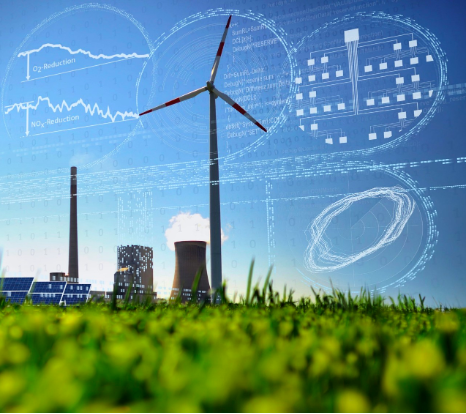
\includegraphics[width=0.6\textwidth, clip, trim={0cm 0cm 0cm 0cm}]{FrontMatter/Cover/Cover}
                	}
%        	\vspace*{1.0cm}
        \end{figure}



        %% Additional whitespace for ease of eye
        \vspace*{2\bigskipamount}


         %% Text color is changed for readability
        \color{white}

        %% Print the name of the author.
        {\makeatletter
                \largetitlefont\Large\bfseries
                \largetitlestyle\fontsize{24}{13cm}\selectfont\@firstname~\@lastname
                \makeatother}


        %% Additional whitespace for ease of eye
        \vspace*{2\bigskipamount}
        \end{center}


\end{titlepage}

%%%% Titlepages
%%%%%%%%%%%%%%%%%%%%%%%%%%%%%%%%%%%%%%%%%%%%%%%%%%
%%%%		~~~~ EDITOR'S NOTE ~~~~
%% 
%% This file contains the title pages in the required Utrecht University format
%% - formal required text fields are included
%%
%% This is the PhD thesis of Laurens P. Stoop in LaTeX
%% - Comments, remarks and more: email me at laurensstoop@protonmail.com
%%
%%%%%%%%%%%%%%%%%%%%%%%%%%%%%%%%%%%%%%%%%%%%%%%%%%



%% This enviroment is called as the titlepage is spread over 4 pages and therefore required
\begin{titlepage}



%%%%%%%%%%%%%%%%%%%%%%%%%%%%%%%%%%%%%%%%%%%%%%%%%%
%%%% ~~~~ Page 1 (base titlepage) ~~~~
%%%%%%%%%%%%%%%%%%%%%%%%%%%%%%%%%%%%%%%%%%%%%%%%%%

%% Centered title page, first page always is without style elements
\begin{center}

        %% Some whitespace at the top.
        \vspace*{2\bigskipamount}



        %%%% Title (bold and big)
        %% To make the title fit better it could be benificial to change \Huge to \huge, \LARGE or even \Large
        {\makeatletter
                \titlestyle\bfseries\Huge\@title
                \makeatother}

        %%%% Optional subtitle.
        %% To make the subtitle fit better it could be benificial to change \LARGE to \Large or \large
        {\makeatletter
                \ifx\@subtitle\undefined\else
                \bigskip
                \titlefont\titleshape\LARGE\@subtitle
                \fi
                \makeatother}



        %% Fill out the page
        \vfill



        %%%% Author (bold is traditional)
        %% To make the name fit better it could be benificial to change \LARGE to \Large or \large
        {\makeatletter
                \titlestyle\bfseries\LARGE\@firstname~{\titleshape\@lastname}
                \makeatother}



        %% Extra whitespace at the bottom.
        \vspace*{4\bigskipamount}

%% End center
\end{center}





%%%%%%%%%%%%%%%%%%%%%%%%%%%%%%%%%%%%%%%%%%%%%%%%%%
%%%% ~~~~ Page 3 (verso with CIP data) ~~~~
%%%%%%%%%%%%%%%%%%%%%%%%%%%%%%%%%%%%%%%%%%%%%%%%%%

%% Force a right page
\cleardoublepage

%% Dedication setting
% - The (optional) dedication can be used to thank someone or display a significant quotation.
% - a empty & clear page is needed
% \clearpage
\thispagestyle{empty}
%% page 350, Lothlorien, last paragraph of the section
\dedication{\epigraph{Science is a wonderful thing \\ if one does not have to earn one's living at it.}{Albert Einstein}}





%%%%%%%%%%%%%%%%%%%%%%%%%%%%%%%%%%%%%%%%%%%%%%%%%%
%%%% ~~~~ Page 4 (verso with CIP data) ~~~~
%%%%%%%%%%%%%%%%%%%%%%%%%%%%%%%%%%%%%%%%%%%%%%%%%%

%% Empty page style as we don't want numbers
\thispagestyle{empty}

%% The information is traditionally listed near the bottom
\vspace*{\fill}


%%%% Research School logo's
%% Inclusion of logos of research schools (not sure if allowed)
\begin{center}
        % 
\includegraphics[height=0.5in]{FrontMatter/Logos/nwo}
        \hfill 
\includegraphics[height=0.5in]{FrontMatter/Logos/sikskleur}
\end{center}


%%%% Research school statement
%% Include the following lines (or something similair) if the dissertation is part of a series
\noindent SIKS Dissertation Series No. XXX \\
The research reported in this thesis has been carried out under the auspices of SIKS, the Dutch Research School for Information and Knowledge Systems.

%% Additional whitespace for ease of eye
\vspace{4\medskipamount}



%%%% CIP information
%% Listing of book information (i.e. ISBN, printerlisting ussualy required by company, credit for cover, digital location)
\noindent
\begin{tabular}{@{}p{0.3\textwidth}@{}p{0.65\textwidth}}
        \textit{ISBN:} &  000-00-0000-000-0 \\[\medskipamount]
        \textit{Printed by:} & Johannes Gutenberg \\[\medskipamount]
        \textit{Cover by:} & Beautiful preliminary cover sketch by Talia \\[\medskipamount]
        \textit{Digital version:} & available at \url{https://dspace.library.uu.nl/}.
\end{tabular}

%% Additional whitespace for ease of eye
\medskip



%%%% Recycled paper use
%% Statement if 100\% recycled paper is used
\noindent This dissertation was printed in limited volume on 100\% recycled paper in an effort to minimize the enviromental footprint.

%% Additional whitespace for ease of eye
\vspace{4\medskipamount}



%%%% Copyright information
%% Could also be inserted manually around the change of the calander year
\noindent Copyright \textcopyright\ \the\year{} by {\makeatletter\@firstname~\@lastname \makeatother}

%%%% More restricting copyright statement
%% N.B.:This is very relevant if part is unpublished
All rights reserved. No part of this publication may be reproduced, stored in a retrieval system or transmitted in any form without the written permission of the copyright owner.






%%%%%%%%%%%%%%%%%%%%%%%%%%%%%%%%%%%%%%%%%%%%%%%%%%
%%%% ~~~~ Page 5 (Formal titlepage) ~~~~
%%
%% NB: While the contents here are dictated by regulations, the styling is not
%%
%%%%%%%%%%%%%%%%%%%%%%%%%%%%%%%%%%%%%%%%%%%%%%%%%%


%% Go to new page by forcing to clear all floats
\clearpage

%% Empty page style as we don't want numbers
\thispagestyle{empty}

%% Center the text
\begin{center}

        %% some whitespace at the top
        \vspace*{2\bigskipamount}

        %% Print the title (original language).
        {\makeatletter
                \titlestyle\bfseries\Huge\@title
                \makeatother}

        %% Print the optional subtitle.
        {\makeatletter
                \ifx\@subtitle\undefined\else
                \bigskip
                \titlefont\titleshape\LARGE\@subtitle
                \fi
                \makeatother}

        %% Flush the rest of the page to the bottom
        \vfill

        %% If original title in not-dutch, provide it in Dutch.
        {\LARGE\titlefont\bfseries Een snelle start van je PhD manuscript}

        %% Also provide a dutch optional sub-title
        {\Large\titlefont\titleshape of een benadering vanuit meerdere hoeken}

        %%%% Required to state that it includes a summary
        %% in Dutch if body not in Dutch
        %% in English if body in Dutch
        (met een samenvatting in het Nederlands)

        %% Include some whitespace
        \bigskip
        \bigskip

        
        {\Large\titlefont Proefschrift}

        %% Include some whitespace
        \bigskip
        \bigskip


        %%%% Required text by the doctoral degree regulations
        %% NB: be very mindfull of the lower case lettering used!!!
        %% NB: basically; do not change this bit
        ter verkrijging van de graad van doctor aan de Universiteit Utrecht\\[\medskipamount]
        op gezag van de rector magnificus, prof.dr.\ H.R.B.M.~Kummeling,\\[\medskipamount]
        ingevolge het besluit van het college voor promoties\\[\medskipamount]
        in het openbaar te verdedigen\\[\medskipamount]
        %%%% Change to relevant date for defense
        %% written as: dayofweek(text) date(number) month(text)  year(number)
        %% if in the morning use: des ochtends te XX.XX uur (use 12-hour format)
        %% if in the afternoon use: des middags te XX.XX uur (use 12-hour format)
        op woensdag DD mmmmm YYYY  des ochtends te UU.UU uur

        %% Include some whitespace
        \bigskip
        \bigskip

        door

        %% Include some whitespace
        \bigskip
        \bigskip



        %%%% Full name
        %% Print the full name of the author.
        {\makeatletter
        \Large\titlefont\bfseries\@firstname~{\titleshape\@lastname}
        \makeatother}



        %% Include some whitespace
        \bigskip
        \bigskip



        %%%% Change to relevant date of birth and town
        %% NB: include country if not born in the Netherlands
        geboren op DD month YYYY te CITY


        %% Extra whitespace at the bottom.
        \vspace*{2\bigskipamount}

\end{center}






%%%%%%%%%%%%%%%%%%%%%%%%%%%%%%%%%%%%%%%%%%%%%%%%%%
%%%%            ~~~~ Page 6 (co-promotor listing) ~~~~
%%
%% NB: contents here are dictated by regulations; CHECK THEM
%%
%%%%%%%%%%%%%%%%%%%%%%%%%%%%%%%%%%%%%%%%%%%%%%%%%%

%% Go to new page by forcing to clear all floats
\clearpage

%% Empty page style as we don't want numbers
\thispagestyle{empty}



%% List the (co-)promotors.
% NB: Only use the title + initials + lastname
Promotoren: \\[\medskipamount] 
\begin{tabular}{@{}p{0.45\textwidth}@{}p{0.50\textwidth}}     
        \textit{Prof.\,dr.\ I.M.~portant} &  Utrecht University \\[\medskipamount]     
\end{tabular}

Copromotoren: \\[\medskipamount] 
\begin{tabular}{@{}p{0.45\textwidth}@{}p{0.50\textwidth}} 
        \textit{dr.\ O.~ther} &  Utrecht University \\[\medskipamount]
\end{tabular}

%% Extra whitespace at the bottom.
\vspace*{2\bigskipamount}



%%%% Assessment committe (in alphabetical order)
%% NB: Only use the title + initials + lastname
Beoordelingscommissie: \\[\medskipamount] 
\begin{tabular}{@{}p{0.45\textwidth}@{}p{0.50\textwidth}}           
        \textit{Prof.\,dr. E.~Smith} &  Unseen University \\[\medskipamount]   
        \textit{Prof.\,dr. H.J.~Farnsworth} &  Mars University \\[\medskipamount]
        \textit{dr. S.~Omega} &  Sigma University \\[\medskipamount]
        \textit{Prof.\,dr. P.~Psi} & University of Longbottom \\[\medskipamount]
        \textit{prof.\,dr. C.~Xi} & Franeker University\\[\medskipamount]
\end{tabular}




%% Flush the rest of the information to the bottom
\vfill

%% Extra whitespace at the bottom.
\vspace*{2\bigskipamount}

%% Example of a financial support statement
\noindent This work was supported by the research project \emph{A Very Important Project} (MAVIP), which was financed by the Some Important Scientific Research Organisation under grant number 011.235.813 and supported by the stakeholder Important Stakeholder\ts{TM}.


%% End of titlepages
\end{titlepage}



%%%% Table of Contents
%% - Set depth of ToC  at this point to 1
%% - Start all counters after the ToC
\setcounter{tocdepth}{1}
\tableofcontents
\startcontents

%%%% Acronym listing (opt)
\printacronyms
\addcontentsline{toc}{chapter}{Acronyms}
\setheader{Acronyms}

%%% Prologue or preface (opt)
%%%%%%%%%%%%%%%%%%%%%%%%%%%%%%%%%%%%%%%%%%%%%%%%%%
%%%%		~~~~ EDITOR'S NOTE ~~~~
%%%%%%%%%%%%%%%%%%%%%%%%%%%%%%%%%%%%%%%%%%%%%%%%%%
%
% This file contains the optional preface of the dissertation
%                       - If included, it's recommended to keep it to 1.5 pages maximum.
%                       - Stylistically the preface is signed & dated
%
% This is the PhD thesis of Laurens P. Stoop in LaTeX
%                       - Comments, remarks and more: email me at laurensstoop@protonmail.com
%
%%%%%%%%%%%%%%%%%%%%%%%%%%%%%%%%%%%%%%%%%%%%%%%%%%
%%%%	 	 ~~~~ END OF: EDITOR'S NOTE ~~~~
%%%%%%%%%%%%%%%%%%%%%%%%%%%%%%%%%%%%%%%%%%%%%%%%%%



%%%%%%%%%%%%%%%%%%%%%%%%%%%%
%%%%            ~~~~ Preface ~~~~
%%%%%%%%%%%%%%%%%%%%%%%%%%%%

%% FrontMatter chapters are unlabeled, but part of the ToC
\chapter*{Preface}
% We add it to the ToC
\addcontentsline{toc}{chapter}{Preface}
% We set the header text
\setheader{Preface}

\emph{Preface goes here. This chapter is optional.}

%% Dumps Lorem-Ipsum
\lipsum[42-49]


%% Automatic signature
%       - change to static information if wanted
%       - italics are normally used
\begin{flushright}
{\makeatletter\itshape
    \@firstname\ \@lastname \\
    Utrecht, \monthyeardate\today
\makeatother}
\end{flushright}







%% Force clear pages to make it neat
\cleardoublepage


%%%%%%%%%%%%%%%%%%%%%%%%%%%%%%%%%%%%%%%%%%%%%%%%%%
%%%% ~~~~ MainMatter ~~~~
%% i.e. the core chapters with an introduction and conclusion
%%
%% - Introduction
%% - Core chapters
%% - Conclusion
%%
%% Here parts are used to provide additional structure to the thesis, this is optional
%%
%% N.B.: No chapter TOC is used for the introduction
%%%%%%%%%%%%%%%%%%%%%%%%%%%%%%%%%%%%%%%%%%%%%%%%%%

%%%% Main Matter style settings
%% Use Arabic numerals for the page numbers of the chapters.
\pagenumbering{arabic}

%% Turn on thumb indices.
%% Make sure to initialize the thumbcounter to the desired initial
%% value using the \setcounter command immediately after turning
%% thumb indices on for the first time.
\thumbtrue



%%%%%%%%%%%%%%%%%%%%%%%%%%%%%%%%%%%%%%%%%%%%%%%%%%
%%%% ~~~~ PART I ~~~~ INTRODUCTION
%%
%% - Introduction
%% - Context / theoretical background
%% - Researhc questions / structure
%%%%%%%%%%%%%%%%%%%%%%%%%%%%%%%%%%%%%%%%%%%%%%%%%%

%%%% Part-title and properties
%% Progress the thumbcounter
\setcounter{thumbcounter}{1}
%% Colour to use for this part
\setcounter{colorcounter}{1}
%% Name and label
\part[Introduction title in the TOC]{Introduction title on the chapter titlepage}
\label{part:intro}



%%%% Qoute
\epigraph{
       You're only given a little spark of madness, and if you lose that... \\ you're nothing.
}{Robin Williams}

%%%% PLAIN LANGUAGE SUMMARY
\section*{Plain Language Summary}
This thesis describes the design, application and evaluation of metrics and measures aimed to support stakeholders to achieve something awesome. 

We show off some cool findings, like the specifc method we used.

Several new techniques have also been explored. 
This meant that we could provide more in-depth insight where it was needed. 

%%%% Part table of contents
\newpage
\chaptoc




%%%% Introduction
%% General introduction to the thesis
%%%%%%%%%%%%%%%%%%%%%%%%%%%%%%%%%%%%%%%%%%%%%%%%%%
%%%%		~~~~ EDITOR'S NOTE ~~~~
%%%%%%%%%%%%%%%%%%%%%%%%%%%%%%%%%%%%%%%%%%%%%%%%%%
%
% This file contains the introduction
%
% This is the PhD thesis of Laurens P. Stoop in LaTeX
%                       - Comments, remarks and more: email me at laurensstoop@protonmail.com
%
%%%%%%%%%%%%%%%%%%%%%%%%%%%%%%%%%%%%%%%%%%%%%%%%%%
%%%%	 	 ~~~~ END OF: EDITOR'S NOTE ~~~~
%%%%%%%%%%%%%%%%%%%%%%%%%%%%%%%%%%%%%%%%%%%%%%%%%%



%%%%%%%%%%%%%%%%%%%%%%%%%%%%
%%%%            ~~~~ Introduction ~~~~
%%%%%%%%%%%%%%%%%%%%%%%%%%%%

\chapter{Introduction}\label{ch:Introduction}

This is a introduction chapter explaining the scientific and technical questions that are currently unsolved.

This line is merely intended to use as a reference to some acronyms used in the main text like \ac{eu} and when used again \ac{eu}.

%% Dumps Lorem-Ipsum
\lipsum[1]

\section{Some context}
%% Dumps Lorem-Ipsum
\lipsum[2-4]





%% Force clear pages to make it neat
\cleardoublepage



%%%%%%%%%%%%%%%%%%%%%%%%%%%%%%%%%%%%%%%%%%%%%%%%%%
%%%% ~~~~ PART II ~~~~ Methods and metrics
%%
%% - Paper 1: Properties of this LaTeX class
%% - Paper 2: A filler chapter
%% - Paper 3: Some filler chapter
%%%%%%%%%%%%%%%%%%%%%%%%%%%%%%%%%%%%%%%%%%%%%%%%%%



%%%% Part-title and properties
%% Progress the thumbcounter
\stepcounter{thumbcounter}
\setcounter{thumbcounter}{20}
%% Colour to use for this part
\setcounter{colorcounter}{2}
%% Name and label
\part[Properties of a dissertation class]{Properties of a dissertation class}
\label{part:second}

%%%% Qoute
\epigraph{
       If you like quotes..  \\ this might be a way to go.
}{Laurens P. Stoop}

%%%% PLAIN LANGUAGE SUMMARY
\section*{Plain Language Summary}
This thesis describes the design, application and evaluation of metrics and measures aimed to support the integration of Energy  \& Climate modelling. aimed to capture relevant aspects of the weather and claimte f. Several new measurement techniques are presented as well as an Application-Specific Integrated Circuit (ASIC) designed for accurate measurement of flow velocity with matrix transducers.

The influence of circuit topologies on the zero-flow performance of ultrasonic flow meters has been analyzed and an algorithm is presented to reduce the offset. With a linear transducer array, flow measurements have been performed via two different acoustic paths, demonstrating the ability to accurately measure flow with array transducers through a stainless-steel pipe wall. In order to improve signal quality, an ASIC has been designed that is able to drive and read-out 96 piezo transducer elements. The ASIC has been characterized electrically and flow measurements have been performed in combination with the linear transducer arrays.

Several new techniques, enabled using transducer arrays, have also been explored. By tapering the amplitude of the transmit signals, spurious waves can be suppressed. An auto-calibration technique has been developed that uses additional acoustic measurements to estimate the diameter of the pipe and the speed of sound in the pipe wall and liquid. Finally, a simulation study has been performed to explore the possibility of exploiting the beam-steering capabilities of transducer arrays to measure flow velocity profiles by using measurements obtained via multiple acoustic paths.


% Set part table of contents on a new page
\newpage
\chaptoc



%% Include a chapter based on a paper
%%%%%%%%%%%%%%%%%%%%%%%%%%%%%%%%%%%%%%%%%%%%%%%%%%
%%%%		~~~~ EDITOR'S NOTE ~~~~
%% 
%% Paper 2: CP2 CREDI
%%
%% This is the PhD thesis of Laurens P. Stoop in LaTeX
%% - Comments, remarks and more: email me at laurensstoop@protonmail.com
%%
%%%%%%%%%%%%%%%%%%%%%%%%%%%%%%%%%%%%%%%%%%%%%%%%%%

\chapter{Dissertation class description}
\label{chapter_1}

%%%% Published/Review/Submitted as a paper.
\blfootnote{The contents of this chapter are under review at A FANCY JOURNAL, for which a preprint is available on arXiv~\autocite{kudela2010turbulent}.}



%% RODE DRAAD STAAT
\epigraph{
       Everything is possible, the impossible might take two days.
}{\emph{Family motto}}



%% PLAIN LANGUAGE SUMMARY
\section*{Plain Language Summary}
In this chapter the properties of the dissertation class are described. 




%% Start the actual chapter on a new page.
\newpage




%%%%%%%%%%%%%%%%%%%%%%%%%%%%%%%%%%%%%%%%%%%%%%%%%%
%%%% ~~~~ Introduction

\noindent This document is intended to be both an example of the Utrecht University dissertation template for \LaTeX, as well as a short introduction to its use. It is not intended to be a general introduction to \LaTeX{} itself,\footnote{We recommend \url{http://en.wikibooks.org/wiki/LaTeX} as a reference and a starting point for new users.} and we will assume the reader to be familiar with the basics of creating and compiling documents.

Instructions on how to use this template under Windows and Linux, and which \LaTeX{} packages are required, can be found in \texttt{README.txt}.


%%%%%%%%%%%%%%%%%%%%%%%%%%%%%%%%%%%%%%%%%%%%%%%%%%
%%%% ~~~~ Structure
\section{Document Structure}

\dropcap{S}{ince} a dissertation is a substantial document, it is convenient to break it up into smaller pieces. In this template we therefore give every chapter its own file. The chapters (and appendices) are gathered together in \texttt{dissertation.tex}, which is the master file describing the overall structure of the document. \texttt{dissertation.tex} starts with the line

%% We need an empty line before the quote environment to work around a bug in
%% the lettrine package, from which the drop command is derived.
\begin{quote}
\texttt{\textbackslash documentclass\{dissertation\}}
\end{quote}
which loads the dissertation template. The template is based on the \LaTeX{} \texttt{book} document class and stored in \texttt{dissertation.cls}. The document class accepts several comma-separated options. By default, hyperlinks are shown in cyan, which is convenient when reading the dissertation on a computer, but can be expensive when printing. They can be turned black with the \texttt{print} option. This will also turn the headers dark gray instead of cyan. Moreover, it will add a 3~mm bleed around the page including crop marks. This will help the printer with the thumb indices, since they run right up to the page borders. Finally, the \texttt{nativefonts} option can be used to override the automatic font selection (see below).

A dissertation is a big document, which makes it easy to miss warnings about the layout in the \LaTeX{} output. In order to locate problem areas, add the \texttt{draft} option to the \texttt{\textbackslash documentclass} line. This will display a vertical bar in the margins next to the paragraphs that require attention.

The contents of the dissertation are included between the \texttt{\textbackslash begin\{document\}} and \texttt{\textbackslash end\{document\}} commands, and split into three parts by
\begin{enumerate}
\item\texttt{\textbackslash frontmatter}, which uses Roman numerals for the page numbers and is used for the title page and the table of contents;
\item\texttt{\textbackslash mainmatter}, which uses Arabic numerals for the page numbers and is the style for the chapters;
\item\texttt{\textbackslash appendix}, which uses letters for the chapter numbers, starting with `A'.
\end{enumerate}
The title page is defined in \texttt{title.tex} in the \texttt{title} folder and included verbatim with \texttt{\textbackslash include\{title/title\}},\footnote{Note that it is not necessary to specify the file extension.} (see below). Additionally, it is possible to include a preface, containing, for example, the acknowledgements. An example can be found in \texttt{preface.tex}. The table of contents is generated automatically with the \texttt{\textbackslash tableofcontents} command. Chapters are included after \texttt{\textbackslash mainmatter} and appendices after \texttt{\textbackslash appendix}. For example, \texttt{\textbackslash include\{chapter-1/chapter-1\}} includes \texttt{chapter-1.tex}, which contains this introduction.

\section{Title Page}

\dropcap{T}{he} title pages are defined in \texttt{title/title.tex}, which you will have to modify according to your needs. Note that these pages are subject to the requirements of the \emph{promotieregelement} and cannot be changed at will. Apart from the names and dates, most of the Dutch text is dictated literally.

Since the thesis title and name of the author appear several times throughout the document (on the title page, but also in, \emph{e.g.}, the preface and cv), special commands are provided so they only have to be specified once. The title (and optional subtitle) can be specified with

\begin{quote}
\texttt{\textbackslash title[Optional subtitle]\{Title\}}
\end{quote}
The name of the author is specified with
\begin{quote}
\texttt{\textbackslash author\{First name\}\{Last name\}}
\end{quote}
Note that the first and last name are separate arguments, since they may be printed in different font shapes. The \texttt{\textbackslash title} and \texttt{\textbackslash author} commands also ensure that the title and author appear in the metadata of the final PDF.

See \texttt{title/title.tex} for detailed documentation on the comment and layout of the title pages. Logos of institutes that have contributed financially to the dissertation may be included on reverse side of the title page. A few example logos can be found in the \texttt{title/logos} folder.

\section{Chapters}

\dropcap{E}{ach} chapter has its own file. For example, the \LaTeX{} source of this chapter can be found in \texttt{chapter-1.tex}. A chapter starts with the command

\begin{quote}
\texttt{\textbackslash chapter\{Chapter title\}}
\end{quote}
This starts a new page, prints the chapter number and title and adds a link in the table of contents. If the title is very long, it may be desirable to use a shorter version in the page headers and the table of contents. This can be achieved by specifying the short title in brackets:

\begin{quote}
\texttt{\textbackslash chapter[Short title]\{Very long title with many words which could not possibly fit on one line\}}
\end{quote}
Unnumbered chapters, such as the preface, can be created with \texttt{\textbackslash chapter*\{Chapter title\}}. Such a chapter will not show up in the table of contents or in the page header. To create a table of contents entry anyway, add
\begin{quote}
    \texttt{\textbackslash addcontentsline\{toc\}\{chapter\}\{Chapter title\}}
\end{quote}
after the \texttt{\textbackslash chapter} command. To print the chapter title in the page header, add
\begin{quote}
    \texttt{\textbackslash setheader\{Chapter title\}}
\end{quote}

If (parts of) the chapter have already been published elsewhere, it is customary to add a reference. This can be done with the special unnumbered footnote command \texttt{\textbackslash blfootnote}. For example,

\begin{quote}
\texttt{\textbackslash blfootnote\{Parts of this chapter have been published in Annalen der Physik \textbackslash textbf\{324\}, 289 (1906) \textbackslash cite \{Einstein1906\}.\}}
\end{quote}
generates the footnote at the beginning of this chapter. Because this footnote is unnumbered, the \texttt{hyperref} package may throw a warning, which safely be ignored.

If multiple people have contributed significantly to this chapter, they can be lister with the \texttt{\textbackslash authors} command. This can be followed by a quotation using \texttt{\textbackslash epigraph} as shown above. Finally, it is customary for a dissertation to include an abstract for every chapter (except perhaps the introduction). This can be accomplished with the \texttt{abstract} environment. The abstract should be followed by \texttt{\textbackslash newpage} to start the chapter text on a new page.

In a dissertation, each chapter has its own list of references. These can be generated with the special command \texttt{\textbackslash references\{dissertation\}} from \texttt{dissertation.bib} at the end of the chapter. Note that this means that you need to run a command like \texttt{bibtex chapter-1/chapter-1} for each chapter. The bibliography style is specified in \texttt{dissertation.bst}, which is a modified version of \texttt{apsrev4-1.bst} (from REVTeX) designed to also display the titles of referenced articles. The template will automatically generate clickable hyperlinks if a URL or DOI (digital object identifier) is present for the reference. Although it is possible to manage the bibliography by hand, we recommend using EndNote (available from Blackboard) or JabRef (available from \url{http://jabref.sourceforge.net/}).

Chapters are subdivided into sections, subsections, subsubsections, and, optionally, paragraphs and subparagraphs. All can have a title, but only sections and subsections are numbered. As with chapters, the numbering can be turned off by using \texttt{\textbackslash section*\{\ldots\}} instead of \texttt{\textbackslash section\{\ldots\}}, and similarly for the subsection.
\section{\textbackslash section\{\ldots\}}
\subsection{\textbackslash subsection\{\ldots\}}
\subsubsection{\textbackslash subsubsection\{\ldots\}}
\paragraph{\textbackslash paragraph\{\ldots\}}
Lorem ipsum dolor sit amet, consectetur adipisicing elit, sed do eiusmod tempor incididunt ut labore et dolore magna aliqua. Ut enim ad minim veniam, quis nostrud exercitation ullamco laboris nisi ut aliquip ex ea commodo consequat. Duis aute irure dolor in reprehenderit in voluptate velit esse cillum dolore eu fugiat nulla pariatur. Excepteur sint occaecat cupidatat non proident, sunt in culpa qui officia deserunt mollit anim id est laborum.

\section{Fonts and Colors}

\dropcap{T}{he} fonts used by this template depend on which version of \LaTeX{} you use. Regular \LaTeX, \emph{i.e.}, if you compile your document with with \texttt{latex}, \texttt{pslatex} or \texttt{pdflatex}, will use Utopia for text, Fourier for math and Latin Modern for sans-serif and monospaced text. However, if you want to adhere to the TU Delft house style, you will need to use \XeLaTeX, as it supports TrueType and OpenType fonts. Compiling with \texttt{xelatex} will use Bookman Old Style for titles, Tahoma for text, Courier New for monospace and Cambria for math. If you want to use \XeLaTeX, but do not want to use the TU Delft house style fonts, you can add the \texttt{nativefonts} option to the document class.

This template supports the use of drop caps, a large colored initial at the beginning of a chapter or section, via the \texttt{\textbackslash dropcap} command:

\begin{quote}
\texttt{\textbackslash dropcap\{L\}\{orem\} ipsum\ldots}
\end{quote}
The first argument is the capital that will be printed on two lines (in the title color), and the second argument is the rest of the word. Depending on the font, the latter may be printed in small caps.

The corporate colors of the TU Delft are cyan, black and white, available, respectively, via \texttt{\textbackslash color\{{\color{tudelft-cyan}tudelft-cyan}\}}, \texttt{\textbackslash color\{{\color{tudelft-black}tudelft-black}\}} (which differs slightly from the default \texttt{black}) and \texttt{\textbackslash color\{tudelft-white\}}. Apart from these three, the house style defines the basic colors
\begin{itemize}
%% Reduce the separation between the items, since this is just a list of words.
\itemsep 0pt
\parskip 0pt
\item\texttt{\color{tudelft-sea-green}tudelft-sea-green},
\item\texttt{\color{tudelft-green}tudelft-green},
\item\texttt{\color{tudelft-dark-blue}tudelft-dark-blue},
\item\texttt{\color{tudelft-purple}tudelft-purple},
\item\texttt{\color{tudelft-turquoise}tudelft-turquoise} and
\item\texttt{\color{tudelft-sky-blue}tudelft-sky-blue},
\end{itemize}
as well as the accent colors
\begin{itemize}
\itemsep 0pt
\parskip 0pt
\item\texttt{\color{tudelft-lavendel}tudelft-lavendel},
\item\texttt{\color{tudelft-orange}tudelft-orange},
\item\texttt{\color{tudelft-warm-purple}tudelft-warm-purple},
\item\texttt{\color{tudelft-fuchsia}tudelft-fuchsia},
\item\texttt{\color{tudelft-bright-green}tudelft-bright-green} and
\item\texttt{\color{tudelft-yellow}tudelft-yellow}.
\end{itemize}






%% Force clear pages to make it neat
\cleardoublepage


%%%%%%%%%%%%%%%%%%%%%%%%%%%%%%%%%%%%%%%%%%%%%%%%%%
%%%% ~~~~ PART X ~~~~ Conclusion
%%
%% - Introduction to conclusion
%% - Scientific summary of chapters
%% - Conclusion to RQ
%% - General synthesis
%%%%%%%%%%%%%%%%%%%%%%%%%%%%%%%%%%%%%%%%%%%%%%%%%%

%%%% Part-title and properties
%% Progress the thumbcounter
\stepcounter{thumbcounter}
%% Colour to use for this part
\setcounter{colorcounter}{3}
%% Name and label
\part[Concluding remarks]{Concluding Remarks}
\label{part:conclusion}


%%%% Qoute
\epigraph{
       If you like quotes.. \\ this might be a way to go.
}{Laurens P. Stoop}

%%%% PLAIN LANGUAGE SUMMARY
\section*{Plain Language Summary}
\lipsum[1337]


% Set part table of contents on a new page
\newpage
\chaptoc





%% Add the actual conclusion (this can be split into scientific summaryu of chapter, conclusion & outlook)
%%%%%%%%%%%%%%%%%%%%%%%%%%%%%%%%%%%%%%%%%%%%%%%%%%
%%%%		~~~~ EDITOR'S NOTE ~~~~
%%%%%%%%%%%%%%%%%%%%%%%%%%%%%%%%%%%%%%%%%%%%%%%%%%
%
% This file contains a conclusion
%
% This is the PhD thesis of Laurens P. Stoop in LaTeX
%                       - Comments, remarks and more: email me at laurensstoop@protonmail.com
%
%%%%%%%%%%%%%%%%%%%%%%%%%%%%%%%%%%%%%%%%%%%%%%%%%%
%%%%	 	 ~~~~ END OF: EDITOR'S NOTE ~~~~
%%%%%%%%%%%%%%%%%%%%%%%%%%%%%%%%%%%%%%%%%%%%%%%%%%



%%%%%%%%%%%%%%%%%%%%%%%%%%%%
%%%%            ~~~~ Conclusion ~~~~
%%%%%%%%%%%%%%%%%%%%%%%%%%%%

\chapter[Conclusion]{Conclusion}\label{app:chapterx}

This is a concluding chapter explaining the scientific and technical
implications for society of the research findings in considerable detail.


%% Dumps Lorem-Ipsum
\lipsum[1]

\section{Some context}
%% Dumps Lorem-Ipsum
\lipsum[2-4]




%%%% Epilogue (opt)
% \chapter*{Epilogue}
\addcontentsline{toc}{chapter}{Epilogue}
\label{epilogue}

This is an optional epilogue.






%% Force clear pages to make it neat
\cleardoublepage





%%%%%%%%%%%%%%%%%%%%%%%%%%%%%%%%%%%%%%%%%%%%%%%%%%
%%%% ~~~~ Part X+1 Appendices ~~~~
%% i.e. the supplemantary information/material or appendices of the core chapters
%%
%% - References
%% - SI of core chapters
%%
%%%%%%%%%%%%%%%%%%%%%%%%%%%%%%%%%%%%%%%%%%%%%%%%%%

%%%% Appendix style settings
%% Use Arabic numerals for the page numbers, but Alphanumeric numbering of the chapters.
\appendix

%%%% Part-title and properties
%% Progress the thumbcounter
\stepcounter{thumbcounter}
%% Colour to use for this part
\setcounter{colorcounter}{4}
%% Name and label
\part[Appendices]{Appendies}
\label{part:appendix}

%%%% Part table of contents
\chaptoc




%%%% References
%% add to the general TOC
\addcontentsline{toc}{chapter}{References}
%% add to the chapter TOC
\addcontentsline{chaptoc}{chapter}{References}
%% add the references & fix the title style
\printbibliography[title={\color{thumb\arabic{thumbcounter}}References}]





%% Appendix to a chapter
%%%%%%%%%%%%%%%%%%%%%%%%%%%%%%%%%%%%%%%%%%%%%%%%%%
%%%%		~~~~ EDITOR'S NOTE ~~~~
%%%%%%%%%%%%%%%%%%%%%%%%%%%%%%%%%%%%%%%%%%%%%%%%%%
%
% This file contains an example appendix to a chapter
%
% This is the PhD thesis of Laurens P. Stoop in LaTeX
%                       - Comments, remarks and more: email me at laurensstoop@protonmail.com
%
%%%%%%%%%%%%%%%%%%%%%%%%%%%%%%%%%%%%%%%%%%%%%%%%%%
%%%%	 	 ~~~~ END OF: EDITOR'S NOTE ~~~~
%%%%%%%%%%%%%%%%%%%%%%%%%%%%%%%%%%%%%%%%%%%%%%%%%%



%%%%%%%%%%%%%%%%%%%%%%%%%%%%
%%%%            ~~~~ Appendix ~~~~
%%%%%%%%%%%%%%%%%%%%%%%%%%%%


\chapter{addition to chapter x}\label{app:chapterx}

Some profound addition





%% Force clear pages to make it neat
\cleardoublepage



%%%%%%%%%%%%%%%%%%%%%%%%%%%%%%%%%%%%%%%%%%%%%%%%%%
%%%% ~~~~ PART X+2 BackMatter ~~~~
%% i.e. the required components that are not part of the work presented
%%
%% - Samenvatting (Nederlands) [required if thesis in English]
%% - List of Publications
%% - Portfolio or courselist (required for some research schools)
%% - Short Curriculum Vitae
%% - Acknowledgements (opt)
%%
%%%%%%%%%%%%%%%%%%%%%%%%%%%%%%%%%%%%%%%%%%%%%%%%%%

%%%% Part-title and properties
%% Progress the thumbcounter
\stepcounter{thumbcounter}
%% Colour to use for this part
\setcounter{colorcounter}{5}
%% Name and label
\part[Backmatter]{Backmatter}
\label{part:backmatter}


%%%% Qoute
\epigraph{
       A good manuscript is a submitted manuscript. A great manuscript is a published manuscript. A perfect manuscript is neither.
}{Shit Academics Say} % on Twitter @AcademicsSay (Dec 7, 2021)}

%% Part table of contents
\chaptoc




%% Samenvatting
%%%%%%%%%%%%%%%%%%%%%%%%%%%%%%%%%%%%%%%%%%%%%%%%%%
%%%%		~~~~ EDITOR'S NOTE ~~~~
%%
%% This file contains an a base fot the Dutch Samenvating
%% - A summary in Dutch is required if the dissertation is not
%% - NB: keep in mind the language setting!
%% 
%% This is the PhD thesis of Laurens P. Stoop in LaTeX
%%                       - Comments, remarks and more: email me at laurensstoop@protonmail.com
%%
%%%%%%%%%%%%%%%%%%%%%%%%%%%%%%%%%%%%%%%%%%%%%%%%%%


%%%%%%%%%%%%%%%%%%%%%%%%%%%%
%%%%            ~~~~ Samenvatting ~~~~
%%%%%%%%%%%%%%%%%%%%%%%%%%%%

\chapter{Nederlandse samenvatting}
%\addcontentsline{toc}{chapter}{Samenvatting}
%\addcontentsline{chaptoc}{chapter}{Samenvatting}
%\setheader{Samenvatting}

%% Correct language setting for line-breaks & typo's
{\selectlanguage{dutch}



Samenvatting in het Nederlands\ldots







%%%%%%%%%%%%%%%%%%%%%%%%%%%%%%%%%%%%%%%%%%%%%%%%%%
%%%% ~~~~ Introduction
% Intro CC -> energy transition
% Humanity is changing Earth's climate.
% Immediate and strong mitigation of climate change is required across all sectors of society, otherwise we will miss the brief and rapidly closing window to secure a liveable future.
% Within the energy sector, a transition towards sustainable resources is already starting to take shape and accelerate.
% This transition increases the impact weather can have on the energy system operations and introduces an additional source of variability in energy systems.
% Knowledge on the emerging compound energy-meteorological variability is required to support the policy makers, energy system planners, and operators around the world that are guiding the energy transition.


%%%%%%%%%%%%%%%%%%%%%%%%%%%%%%%%%%%%%%%%%%%%%%%%%%
%%%% ~~~~ Part I Challenges and RQ

\subsection*{Onderzoeksvraag}
% % Aim of thesis
% This thesis aims to contribute to tackling some of the open research challenges in this field by providing data driven insight into the relevant impact of energy-meteorological variability on energy system operation, specifically for the use of energy system planners and policymakers.
% To do this, techniques from algorithmic data analysis are combined with knowledge on energy and resources, as well as an understanding of the driving physical forces of the weather and climate.

% % structure
% This thesis consists of two parts: the first delves into data driven methods and measures to gain a better understanding of energy-meteorological variability; the second discusses methods to integrate this understanding in energy system operations.


%%%%%%%%%%%%%%%%%%%%%%%%%%%%%%%%%%%%%%%%%%%%%%%%%%
%%%% ~~~~ Part II Metrics and measures
\subsection*{Data gedreven maatstaven}
% % Part 1: Data driven methods
% In the first part, three papers are presented that aim to determine and apply relevant data driven methods and approaches to quantify and understand the energy-meteorological variability present in future power systems and the critical, high impact due to this variability.

% % CS1
% The first paper discusses an outlier detection technique, i.e. the Maximum Divergent Intervals algorithm, to systematically find critical, high impact events that are relevant for energy system reliability.
% Furthermore, it discusses the properties of the events found over a 70-year historical period.

% % CP2
% The second paper develops the Climatological Renewable Energy Deviation Index that can be used to quantify energy-meteorological variability across timescales, and discusses its use for researchers and stakeholders to assess the impact of energy-meteorological variability in energy system operation.

% % MSc1
% The third paper contains an investigation into extreme impacts of energy-meteorological variability on a future energy system using a large -- 3$\times$2000 years -- climate simulation dataset, and presents a characterisation of the 1-, 7-, and 14-day duration events found.

%%%%%%%%%%%%%%%%%%%%%%%%%%%%%%%%%%%%%%%%%%%%%%%%%%
%%%% ~~~~ Part III towards integration
\subsection*{Integratie van veranderlijkheid in operatie}
% % Part 2: Towards understanding
% In the second part, two papers are presented that aim to integrate the understanding, and the representation, of energy-meteorological variability with operational energy system models to address knowledge gaps for those guiding the energy transition.

% % CP1
% The first paper presents an investigation on the relation between critical moments in an operational power system model, defined through energy not served, and large scale weather patterns based on the available 28 years of historical weather and 12 scenarios of a future European power system.
% It highlights the relation between structural shortage and some of the prevailing weather patterns in the winter period.

% % Ext1
% The second paper presents a post-processing method to investigate the effect of climate change on the adequacy of the European power system, and as it shows a significant effect, it highlights the importance of incorporating climate change in adequacy assessments.

%%%%%%%%%%%%%%%%%%%%%%%%%%%%%%%%%%%%%%%%%%%%%%%%%%
%%%% ~~~~ Part IV Synthesis
\subsection*{Synthese van het begrip in de dagelijkse werkelijkheid}
% % Conclusion
% In this thesis a number of data driven methods to increase the understanding of energy-meteorological variability and its impact on energy system operations are shown.
% By studying the existing algorithms, methods and models from the overlapping perspective of an energy-, climate-, and data scientist, transdisciplinary approaches have been developed to provide the understanding needed for grounded decisions by researchers and stakeholders in the power sector.

% % practical application


% % interdisciplinarity
% The presented results within this thesis are the product of an inter- and transdisciplinary research effort, and the findings of this thesis are as interconnected as the disciplines that informed them.
%%%%%% JOKE ON BUZZ-WORDINESS









%% Closing bracket of the language setting
}




%% Turn off thumb indices for unnumbered chapters.
%               - It's a style choice where you turn these off
\thumbfalse


%%%% List of SIKS dissertations
%% Required for SIKS
%%%%%%%%%%%%%%%%%%%%%%%%%%%%%%%%%%%%%%%%%%%%%%%%%%
%%%%		~~~~ EDITOR'S NOTE ~~~~
%%
%% This file contains the list of SIKS-disserations
%% - an overview of this is required for a SIKS-dissertation
%% 
%% This is the PhD thesis of Laurens P. Stoop in LaTeX
%%                       - Comments, remarks and more: email me at laurensstoop@protonmail.com
%%
%%%%%%%%%%%%%%%%%%%%%%%%%%%%%%%%%%%%%%%%%%%%%%%%%%

%% Name
\chapter{List of SIKS-dissertations }
\label{siks}



{\small

\section*{2016}
\begin{xltabular}{\linewidth}{@{} l @{\hspace{0.5em}} l @{\hspace{1em}} X @{}}

         \toprule
        2016
        &	 01	&	 Syed Saiden Abbas (RUN), Recognition of Shapes by Humans and Machines\\
        &	 02	&	 Michiel Christiaan Meulendijk (UU), Optimizing medication reviews through decision support: prescribing a better pill to swallow\\
        &	 03	&	 Maya Sappelli (RUN), Knowledge Work in Context: User Centered Knowledge Worker Support\\
        &	 04	&	 Laurens Rietveld (VU), Publishing and Consuming Linked Data\\
        &	 05	&	 Evgeny Sherkhonov (UVA), Expanded Acyclic Queries: Containment and an Application in Explaining Missing Answers\\
        &	 06	&	 Michel Wilson (TUD), Robust scheduling in an uncertain environment\\
        &	 07	&	 Jeroen de Man (VU), Measuring and modeling negative emotions for virtual training\\
        &	 08	&	 Matje van de Camp (TiU), A Link to the Past: Constructing Historical Social Networks from Unstructured Data\\
        &	 09	&	 Archana Nottamkandath (VU), Trusting Crowdsourced Information on Cultural Artefacts\\
        &	 10	&	 George Karafotias (VUA), Parameter Control for Evolutionary Algorithms\\
        &	 11	&	 Anne Schuth (UVA), Search Engines that Learn from Their Users\\
        &	 12	&	 Max Knobbout (UU), Logics for Modelling and Verifying Normative Multi-Agent Systems\\
        &	 13	&	 Nana Baah Gyan (VU), The Web, Speech Technologies and Rural Development in West Africa - An ICT4D Approach\\
        &	 14	&	 Ravi Khadka (UU), Revisiting Legacy Software System Modernization\\
        &	 15	&	 Steffen Michels (RUN), Hybrid Probabilistic Logics - Theoretical Aspects, Algorithms and Experiments\\
        &	 16	&	 Guangliang Li (UVA), Socially Intelligent Autonomous Agents that Learn from Human Reward\\
        &	 17	&	 Berend Weel (VU), Towards Embodied Evolution of Robot Organisms\\
        &	 18	&	 Albert Mero\~{n}o Pe\~{n}uela (VU), Refining Statistical Data on the Web\\
        &	 19	&	 Julia Efremova (Tu/e), Mining Social Structures from Genealogical Data\\
        &	 20	&	 Daan Odijk (UVA), Context \& Semantics in News \& Web Search\\
        &	 21	&	 Alejandro Moreno C\'{e}lleri (UT), From Traditional to Interactive Playspaces: Automatic Analysis of Player Behavior in the Interactive Tag Playground\\
        &	 22	&	 Grace Lewis (VU), Software Architecture Strategies for Cyber-Foraging Systems\\
        &	 23	&	 Fei Cai (UVA), Query Auto Completion in Information Retrieval\\
        &	 24	&	 Brend Wanders (UT), Repurposing and Probabilistic Integration of Data; An Iterative and data model independent approach\\
        &	 25	&	 Julia Kiseleva (TU/e), Using Contextual Information to Understand Searching and Browsing Behavior\\
        &	 26	&	 Dilhan Thilakarathne (VU), In or Out of Control: Exploring Computational Models to Study the Role of Human Awareness and Control in Behavioural Choices, with Applications in Aviation and Energy Management Domains\\
        &	 27	&	 Wen Li (TUD), Understanding Geo-spatial Information on Social Media\\
        &	 28	&	 Mingxin Zhang (TUD), Large-scale Agent-based Social Simulation - A study on epidemic prediction and control\\
        &	 29	&	 Nicolas H\"{o}ning (TUD), Peak reduction in decentralised electricity systems - Markets and prices for flexible planning\\
        &	 30	&	 Ruud Mattheij (UvT), The Eyes Have It\\
        &	 31	&	 Mohammad Khelghati (UT), Deep web content monitoring\\
        &	 32	&	 Eelco Vriezekolk (UT), Assessing Telecommunication Service Availability Risks for Crisis Organisations\\
        &	 33	&	 Peter Bloem (UVA), Single Sample Statistics, exercises in learning from just one example\\
        &	 34	&	 Dennis Schunselaar (TUE), Configurable Process Trees: Elicitation, Analysis, and Enactment\\
        &	 35	&	 Zhaochun Ren (UVA), Monitoring Social Media: Summarization, Classification and Recommendation\\
        &	 36	&	 Daphne Karreman (UT), Beyond R2D2: The design of nonverbal interaction behavior optimized for robot-specific morphologies\\
        &	 37	&	 Giovanni Sileno (UvA), Aligning Law and Action - a conceptual and computational inquiry\\
        &	 38	&	 Andrea Minuto (UT), Materials that Matter - Smart Materials meet Art \& Interaction Design\\
        &	 39	&	 Merijn Bruijnes (UT), Believable Suspect Agents; Response and Interpersonal Style Selection for an Artificial Suspect\\
        &	 40	&	 Christian Detweiler (TUD), Accounting for Values in Design\\
        &	 41	&	 Thomas King (TUD), Governing Governance: A Formal Framework for Analysing Institutional Design and Enactment Governance\\
        &	 42	&	 Spyros Martzoukos (UVA), Combinatorial and Compositional Aspects of Bilingual Aligned Corpora\\
        &	 43	&	 Saskia Koldijk (RUN), Context-Aware Support for Stress Self-Management: From Theory to Practice\\
        &	 44	&	 Thibault Sellam (UVA), Automatic Assistants for Database Exploration\\
        &	 45	&	 Bram van de Laar (UT), Experiencing Brain-Computer Interface Control\\
        &	 46	&	 Jorge Gallego Perez (UT), Robots to Make you Happy\\
        &	 47	&	 Christina Weber (UL), Real-time foresight - Preparedness for dynamic innovation networks\\
        &	 48	&	 Tanja Buttler (TUD), Collecting Lessons Learned\\
        &	 49	&	 Gleb Polevoy (TUD), Participation and Interaction in Projects. A Game-Theoretic Analysis\\
        &	 50	&	 Yan Wang (UVT), The Bridge of Dreams: Towards a Method for Operational Performance Alignment in IT-enabled Service Supply Chains\\

% \bottomrule
\end{xltabular}


\section*{2017}
\begin{xltabular}{\linewidth}{@{} l @{\hspace{0.5em}} l @{\hspace{1em}} X @{}}

        \toprule
        2017
        &	 01	&	 Jan-Jaap Oerlemans (UL), Investigating Cybercrime\\
        &	 02	&	 Sjoerd Timmer (UU), Designing and Understanding Forensic Bayesian Networks using Argumentation\\
        &	 03	&	 Dani\"{e}l Harold Telgen (UU), Grid Manufacturing; A Cyber-Physical Approach with Autonomous Products and Reconfigurable Manufacturing Machines\\
        &	 04	&	 Mrunal Gawade (CWI), Multi-core Parallelism in a Column-store\\
        &	 05	&	 Mahdieh Shadi (UVA), Collaboration Behavior\\
        &	 06	&	 Damir Vandic (EUR), Intelligent Information Systems for Web Product Search\\
        &	 07	&	 Roel Bertens (UU), Insight in Information: from Abstract to Anomaly\\
        &	 08	& 	 Rob Konijn (VU)	, Detecting Interesting Differences:Data Mining in Health Insurance Data using Outlier Detection and Subgroup Discovery\\
        &	 09	&	 Dong Nguyen (UT), Text as Social and Cultural Data: A Computational Perspective on Variation in Text\\
        &	 10	&	 Robby van Delden (UT), (Steering) Interactive Play Behavior\\
        &	 11	&	 Florian Kunneman (RUN), Modelling patterns of time and emotion in Twitter \#anticipointment\\
        &	 12	&	 Sander Leemans (TUE), Robust Process Mining with Guarantees\\
        &	 13	& 	 Gijs Huisman (UT),  Social Touch Technology - Extending the reach of social touch through haptic technology\\
        &	 14	&	 Shoshannah Tekofsky (UvT), You Are Who You Play You Are: Modelling Player Traits from Video Game Behavior\\
        &	 15	&	 Peter Berck (RUN),  Memory-Based Text Correction\\
        &	 16	&	 Aleksandr Chuklin (UVA), Understanding and Modeling Users of Modern Search Engines\\
        &	 17	&	 Daniel Dimov (UL), Crowdsourced Online Dispute Resolution\\
        &	 18	&	 Ridho Reinanda (UVA), Entity Associations for Search\\
        &	 19	& 	 Jeroen Vuurens (UT), Proximity of Terms, Texts and Semantic Vectors in Information Retrieval\\
        &	 20	&	 Mohammadbashir Sedighi (TUD), Fostering Engagement in Knowledge Sharing: The Role of Perceived Benefits, Costs and Visibility\\
        &	 21	&	 Jeroen Linssen (UT), Meta Matters in Interactive Storytelling and Serious Gaming (A Play on Worlds)\\
        &	 22	&	 Sara Magliacane (VU), Logics for causal inference under uncertainty\\
        &	 23	&	 David Graus (UVA), Entities of Interest --- Discovery in Digital Traces\\
        &	 24	&	 Chang Wang (TUD), Use of Affordances for Efficient Robot Learning\\
        &	 25	&	 Veruska Zamborlini (VU), Knowledge Representation for Clinical Guidelines, with applications to Multimorbidity Analysis and Literature Search\\
        &	 26	&	 Merel Jung (UT), Socially intelligent robots that understand and respond to human touch\\
        &	 27	&	 Michiel Joosse (UT), Investigating Positioning and Gaze Behaviors of Social Robots: People's Preferences, Perceptions and Behaviors\\
        &	 28	&	 John Klein (VU), Architecture Practices for Complex Contexts\\
        &	 29	&	 Adel Alhuraibi (UvT), From IT-BusinessStrategic Alignment to Performance: A Moderated Mediation Model of Social Innovation, and Enterprise Governance of    IT"\\
        &	 30	&	 Wilma Latuny (UvT), The Power of Facial Expressions\\
        &	 31	&	 Ben Ruijl (UL), Advances in computational methods for QFT calculations\\
        &	 32	& 	 Thaer Samar (RUN), Access to and Retrievability of Content in Web Archives\\
        &	 33	&	 Brigit van Loggem (OU), Towards a Design Rationale for Software Documentation: A Model of Computer-Mediated Activity\\
        &	 34	&	 Maren Scheffel (OU), The Evaluation Framework for Learning Analytics \\
        &	 35	&	 Martine de Vos (VU), Interpreting natural science spreadsheets \\
        &	 36	&	 Yuanhao Guo (UL), Shape Analysis for Phenotype Characterisation from High-throughput Imaging \\
        &	 37	&	 Alejandro Montes Garcia (TUE), WiBAF: A Within Browser Adaptation Framework that Enables Control over Privacy \\
        &	 38	&	 Alex Kayal (TUD), Normative Social Applications \\
        &	 39	&	 Sara Ahmadi (RUN), Exploiting properties of the human auditory system and compressive sensing methods to increase   noise robustness in ASR \\
        &	 40	&	 Altaf Hussain Abro (VUA), Steer your Mind: Computational Exploration of Human Control in Relation to Emotions, Desires and Social Support For applications in human-aware support systems \\
        &	 41	&	 Adnan Manzoor (VUA), Minding a Healthy Lifestyle: An Exploration of Mental Processes and a Smart Environment to Provide Support for a Healthy Lifestyle\\
        &	 42	&	 Elena Sokolova (RUN), Causal discovery from mixed and missing data with applications on ADHD  datasets\\
        &	 43	&	 Maaike de Boer (RUN), Semantic Mapping in Video Retrieval\\
        &	 44	&	 Garm Lucassen (UU), Understanding User Stories - Computational Linguistics in Agile Requirements Engineering\\
        &	 45	&	 Bas Testerink	(UU), Decentralized Runtime Norm Enforcement\\
        &	 46	&	 Jan Schneider	(OU), Sensor-based Learning Support\\
        &	 47	&	 Jie Yang (TUD), Crowd Knowledge Creation Acceleration\\
        &	 48	&	 Angel Suarez (OU), Collaborative inquiry-based learning\\

% \bottomrule
\end{xltabular}


\section*{2018}
\begin{xltabular}{\linewidth}{@{} l @{\hspace{0.5em}} l @{\hspace{1em}} X @{}}

        \toprule
        2018
        &	 01	&	 Han van der Aa (VUA), Comparing and Aligning Process Representations \\
        &	 02	&	 Felix Mannhardt (TUE), Multi-perspective Process Mining \\
        &	 03	&	 Steven Bosems (UT), Causal Models For Well-Being: Knowledge Modeling, Model-Driven Development of Context-Aware Applications, and Behavior Prediction\\
        &	 04	&	 Jordan Janeiro (TUD), Flexible Coordination Support for Diagnosis Teams in Data-Centric Engineering Tasks \\
        &	 05	&	 Hugo Huurdeman (UVA), Supporting the Complex Dynamics of the Information Seeking Process \\
        &	 06	&	 Dan Ionita (UT), Model-Driven Information Security Risk Assessment of Socio-Technical Systems \\
        &	 07	&	 Jieting Luo (UU), A formal account of opportunism in multi-agent systems \\
        &	 08	&	 Rick Smetsers (RUN), Advances in Model Learning for Software Systems \\
        &	 09	&	 Xu Xie	(TUD), Data Assimilation in Discrete Event Simulations \\
        &	 10	&	 Julienka Mollee (VUA), Moving forward: supporting physical activity behavior change through intelligent technology \\
        &	 11	&	 Mahdi Sargolzaei (UVA), Enabling Framework for Service-oriented Collaborative Networks \\
        &	 12	&	 Xixi Lu (TUE), Using behavioral context in process mining \\
        &	 13	&	 Seyed Amin Tabatabaei (VUA), Computing a Sustainable Future \\
        &	 14	&	 Bart Joosten (UVT), Detecting Social Signals with Spatiotemporal Gabor Filters \\
        &	 15	&	 Naser Davarzani (UM), Biomarker discovery in heart failure \\
        &	 16	&	 Jaebok Kim (UT), Automatic recognition of engagement and emotion in a group of children \\
        &	 17	&	 Jianpeng Zhang (TUE), On Graph Sample Clustering \\
        &	 18	& 	 Henriette Nakad (UL), De Notaris en Private Rechtspraak \\
        &	 19	&	 Minh Duc Pham (VUA), Emergent relational schemas for RDF \\
        &	 20	&	 Manxia Liu (RUN), Time and Bayesian Networks \\
        &	 21	&	 Aad Slootmaker (OUN), EMERGO: a generic platform for authoring and playing scenario-based serious games \\
        &	 22	&	 Eric Fernandes de Mello Ara\'{u}jo (VUA), Contagious: Modeling the Spread of Behaviours, Perceptions and Emotions in Social Networks \\
        &	 23	&	 Kim Schouten (EUR), Semantics-driven Aspect-Based Sentiment Analysis \\
        &	 24	&	 Jered Vroon (UT), Responsive Social Positioning Behaviour for Semi-Autonomous Telepresence Robots \\
        &	 25	&	 Riste Gligorov (VUA), Serious Games in Audio-Visual Collections \\
        &	 26	& 	 Roelof Anne Jelle de Vries (UT),Theory-Based and Tailor-Made: Motivational Messages for Behavior Change Technology \\
        &	 27	&	 Maikel Leemans (TUE), Hierarchical Process Mining for Scalable Software Analysis \\
        &	 28	&	 Christian Willemse (UT), Social Touch Technologies: How they feel and how they make you feel \\
        &	 29	&	 Yu Gu (UVT), Emotion Recognition from Mandarin Speech \\
        &	 30	&	 Wouter Beek,  The "K" in "semantic web" stands for "knowledge": scaling semantics to the web \\


% \bottomrule
\end{xltabular}


\section*{2019}
\begin{xltabular}{\linewidth}{@{} l @{\hspace{0.5em}} l @{\hspace{1em}} X @{}}

        \toprule
        2019
        &	 01	&	 Rob van Eijk (UL),Web privacy measurement in real-time bidding systems. A graph-based approach to RTB system classification \\
        &	 02	&	 Emmanuelle Beauxis Aussalet (CWI, UU), Statistics and Visualizations for Assessing Class Size Uncertainty \\
        &	 03	&	 Eduardo Gonzalez Lopez de Murillas (TUE), Process Mining on Databases: Extracting Event Data from Real Life Data Sources \\
        &	 04	&	 Ridho Rahmadi (RUN), Finding stable causal structures from clinical data \\
        & 	 05	&	 Sebastiaan van Zelst (TUE), Process Mining with Streaming Data \\
        &	 06	& 	 Chris Dijkshoorn (VU), Nichesourcing for Improving Access to Linked Cultural Heritage Datasets \\
        &	 07	&	 Soude Fazeli (TUD), Recommender Systems in Social Learning Platforms \\
        & 	 08	&	 Frits de Nijs (TUD), Resource-constrained Multi-agent Markov Decision Processes \\
        &	 09	&	 Fahimeh Alizadeh Moghaddam (UVA), Self-adaptation for energy efficiency in software systems \\
        &	 10	&	 Qing Chuan Ye (EUR), Multi-objective Optimization Methods for Allocation and Prediction \\
        &	 11	&	 Yue Zhao (TUD), Learning Analytics Technology to Understand Learner Behavioral Engagement in MOOCs \\
        &	 12	&	 Jacqueline Heinerman (VU), Better Together \\
        &	 13	&	 Guanliang Chen (TUD), MOOC Analytics: Learner Modeling and Content Generation \\
        &	 14	&	 Daniel Davis (TUD), Large-Scale Learning Analytics: Modeling Learner Behavior \& Improving Learning Outcomes in Massive Open Online Courses \\
        &	 15	&	 Erwin Walraven (TUD), Planning under Uncertainty in Constrained and Partially Observable Environments \\
        &	 16	&	 Guangming Li (TUE), Process Mining based on Object-Centric Behavioral Constraint (OCBC) Models \\
        &	 17	&	 Ali Hurriyetoglu (RUN),Extracting actionable information from microtexts \\
        &	 18	&	 Gerard Wagenaar (UU), Artefacts in Agile Team Communication \\
        &	 19	&	 Vincent Koeman (TUD), Tools for Developing Cognitive Agents \\
        &	 20	&	 Chide Groenouwe (UU), Fostering technically augmented human collective intelligence \\
        &	 21	&	 Cong Liu (TUE), Software Data Analytics: Architectural Model Discovery and Design Pattern Detection \\
        &	 22	&	 Martin van den Berg (VU),Improving IT Decisions with Enterprise Architecture \\
        &	 23	&	 Qin Liu (TUD), Intelligent Control Systems: Learning, Interpreting, Verification\\
        &	 24	&	 Anca Dumitrache (VU),  Truth in Disagreement - Crowdsourcing Labeled Data for Natural Language Processing\\
        &	 25	&	 Emiel van Miltenburg (VU), Pragmatic factors in (automatic) image description \\
        &	 26	&	 Prince Singh (UT), An Integration Platform for Synchromodal Transport \\
        &	 27	&	 Alessandra Antonaci (OUN), The Gamification Design Process applied to (Massive) Open Online Courses\\
        &	 28	&	 Esther Kuindersma (UL), Cleared for take-off: Game-based learning to prepare airline pilots for critical situations \\
        &	 29	&	 Daniel Formolo (VU), Using virtual agents for simulation and training of social skills in safety-critical circumstances \\
        &	 30	&	 Vahid Yazdanpanah (UT), Multiagent Industrial Symbiosis Systems \\
        &	 31	&	 Milan Jelisavcic (VU), Alive and Kicking: Baby Steps in Robotics \\
        &	 32	&	 Chiara Sironi (UM), Monte-Carlo Tree Search for Artificial General Intelligence in Games \\
        &	 33	&	 Anil Yaman (TUE), Evolution of Biologically Inspired Learning in Artificial Neural Networks \\
        &	 34	&	 Negar Ahmadi (TUE), EEG Microstate and Functional Brain Network Features for Classification of Epilepsy and PNES \\
        &	 35	&	 Lisa Facey-Shaw (OUN), Gamification with digital badges in learning programming \\
        &	 36	&	 Kevin Ackermans (OUN), Designing Video-Enhanced Rubrics to Master Complex Skills \\
        &	 37	&	 Jian Fang (TUD), Database Acceleration on FPGAs \\
        &	 38	&	 Akos Kadar (OUN), Learning visually grounded and multilingual representations \\


% \bottomrule
\end{xltabular}


\section*{2020}
\begin{xltabular}{\linewidth}{@{} l @{\hspace{0.5em}} l @{\hspace{1em}} X @{}}

        \toprule
        2020
        &	 01	&	 Armon Toubman (UL), Calculated Moves: Generating Air Combat Behaviour \\
        &	 02	&	 Marcos de Paula Bueno (UL), Unraveling Temporal Processes using Probabilistic Graphical Models \\
        &	 03	&	 Mostafa Deghani (UvA), Learning with Imperfect Supervision for Language Understanding \\
        &	 04	&	 Maarten van Gompel (RUN), Context as Linguistic Bridges \\
        &	 05	&	 Yulong Pei (TUE), On local and global structure mining \\
        &	 06	&	 Preethu Rose Anish (UT), Stimulation Architectural Thinking during Requirements Elicitation - An Approach and Tool Support \\
        &	 07	&	 Wim van der Vegt (OUN), Towards a software architecture for reusable game components \\
        &	 08	&	 Ali Mirsoleimani (UL),Structured Parallel Programming for Monte Carlo Tree Search \\
        &	 09	&	 Myriam Traub (UU), Measuring Tool Bias and Improving Data Quality for Digital Humanities Research \\
        &	 10	&	 Alifah Syamsiyah (TUE), In-database Preprocessing for Process Mining \\
        &	 11	&	 Sepideh Mesbah (TUD), Semantic-Enhanced Training Data AugmentationMethods for Long-Tail Entity Recognition Models \\
        &	 12	&	 Ward van Breda (VU), Predictive Modeling in E-Mental Health: Exploring Applicability in Personalised Depression Treatment \\
        &	 13	&	 Marco Virgolin (CWI), Design and Application of Gene-pool Optimal Mixing Evolutionary Algorithms for Genetic Programming \\
        &	 14	&	 Mark Raasveldt (CWI/UL), Integrating Analytics with Relational Databases \\
        &	 15	&	 Konstantinos Georgiadis (OUN),  Smart CAT: Machine Learning for Configurable Assessments in Serious Games \\
        &	 16	&	 Ilona Wilmont (RUN), Cognitive Aspects of Conceptual Modelling \\
        &	 17	&	 Daniele Di Mitri (OUN), The Multimodal Tutor: Adaptive Feedback from Multimodal Experiences \\
        &	 18	&	 Georgios Methenitis (TUD), Agent Interactions \& Mechanisms in Markets with Uncertainties: Electricity Markets in Renewable Energy Systems \\
        &	 19	&	 Guido van Capelleveen (UT), Industrial Symbiosis Recommender Systems \\
        &	 20	&	 Albert Hankel (VU), Embedding Green ICT Maturity in Organisations \\
        &	 21	&	 Karine da Silva Miras de Araujo (VU), Where is the robot?: Life as it could be \\
        &	 22	&	 Maryam Masoud Khamis (RUN), Understanding complex systems implementation through a modeling approach: the case of e-government in Zanzibar \\
        &	 23	&	 Rianne Conijn (UT), The Keys to Writing: A writing analytics approach to studying writing processes using keystroke logging \\
        &	 24	&	 Lenin da N\'{o}brega Medeiros (VUA/RUN), How are you feeling, human? Towards emotionally supportive chatbots \\
        &	 25	&	 Xin Du (TUE), The Uncertainty in Exceptional Model Mining \\
        &	 26	&	 Krzysztof Leszek Sadowski (UU), GAMBIT: Genetic Algorithm for Model-Based mixed-Integer opTimization \\
        &	 27	&	 Ekaterina Muravyeva (TUD), Personal data and informed consent in an educational context \\
        &	 28	&	 Bibeg Limbu (TUD), Multimodal interaction for deliberate practice: Training complex skills with augmented reality \\
        &	 29	&	 Ioan Gabriel Bucur (RUN), Being Bayesian about Causal Inference \\
        &	 30	&	 Bob Zadok Blok (UL), Creatief, Creatieve, Creatiefst \\
        &	 31	&	 Gongjin Lan (VU), Learning better -- From Baby to Better \\
        &	 32	& 	 Jason Rhuggenaath (TUE), Revenue management in online markets: pricing and online advertising \\
        &	 33	& 	 Rick Gilsing (TUE), Supporting service-dominant business model evaluation in the context of business model innovation \\
        &	 34	&	 Anna Bon (MU), Intervention or Collaboration? Redesigning Information and Communication Technologies for Development \\
        &	 35	&	 Siamak Farshidi (UU), Multi-Criteria Decision-Making in Software Production \\

% \bottomrule
\end{xltabular}


\section*{2021}
\begin{xltabular}{\linewidth}{@{} l @{\hspace{0.5em}} l @{\hspace{1em}} X @{}}

        \toprule
        2021
        &	 01	&	 Francisco Xavier Dos Santos Fonseca (TUD),Location-based Games for Social Interaction in Public Space \\
        &	 02	&	 Rijk Mercuur (TUD), Simulating Human Routines: Integrating Social Practice Theory in Agent-Based Models \\
        &	 03	&	 Seyyed Hadi Hashemi (UVA), Modeling Users Interacting with Smart Devices \\
        &	 04	&	 Ioana Jivet (OU), The Dashboard That Loved Me: Designing adaptive learning analytics for self-regulated learning \\
        &	 05	&	 Davide Dell'Anna (UU), Data-Driven Supervision of Autonomous Systems \\
        &	 06	&	 Daniel Davison (UT), "Hey robot, what do you think?" How children learn with a social robot \\
        &	 07	&	 Armel Lefebvre (UU), Research data management for open science \\
        &	 08	&	 Nardie Fanchamps (OU), The Influence of Sense-Reason-Act Programming on Computational Thinking \\
        &	 09	&	 Cristina Zaga (UT), The Design of Robothings. Non-Anthropomorphic and Non-Verbal Robots to Promote Children's Collaboration Through Play \\
        &	 10	&	 Quinten Meertens (UvA), Misclassification Bias in Statistical Learning \\
        &	 11	&	 Anne van Rossum (UL), Nonparametric Bayesian Methods in Robotic Vision \\
        &	 12	&	 Lei Pi (UL), External Knowledge Absorption in Chinese SMEs \\
        &	 13	&	 Bob R. Schadenberg (UT), Robots for Autistic Children: Understanding and Facilitating Predictability for Engagement in Learning \\
        &	 14	&	 Negin Samaeemofrad (UL), Business Incubators: The Impact of Their Support \\
        &	 15	& 	 Onat Ege Adali (TU/e), Transformation of Value Propositions into Resource Re-Configurations through the Business Services Paradigm  \\
        &	 16	&	 Esam A. H. Ghaleb (UM), Bimodal emotion recognition from audio-visual cues \\
        &	 17	&	 Dario Dotti (UM), Human Behavior Understanding  from motion and bodily cues using deep neural networks \\
        &	 18	&	 Remi Wieten (UU), Bridging the Gap Between Informal Sense-Making Tools and Formal Systems - Facilitating the Construction of Bayesian Networks and Argumentation Frameworks \\
        &	 19	&	 Roberto Verdecchia (VU), Architectural Technical Debt: Identification and Management \\
        &	 20	&	 Masoud Mansoury (TU/e), Understanding and Mitigating Multi-Sided Exposure Bias in Recommender Systems \\
        &	 21	&	 Pedro Thiago Timb\'{o} Holanda (CWI), Progressive Indexes \\
        &	 22	&	 Sihang Qiu (TUD), Conversational Crowdsourcing \\
        &	 23	&	 Hugo Manuel Proen\c{c}a (LIACS), Robust rules for prediction and description \\
        &	 24	&	 Kaijie Zhu (TUE), On Efficient Temporal Subgraph Query Processing \\
        &	 25	&	 Eoin Martino Grua (VUA), The Future of E-Health is Mobile: Combining AI and Self-Adaptation to Create Adaptive E-Health Mobile Applications \\
        &	 26	& 	 Benno Kruit (CWI \& VUA), Reading the Grid: Extending Knowledge Bases from Human-readable Tables \\
        &	 27	&	 Jelte van Waterschoot (UT), Personalized and Personal Conversations: Designing Agents Who Want to Connect With You \\
        &	 28	&	 Christoph Selig (UL), Understanding the Heterogeneity of Corporate Entrepreneurship Programs \\

% \bottomrule
\end{xltabular}

\section*{2022}
\begin{xltabular}{\linewidth}{@{} l @{\hspace{0.5em}} l @{\hspace{1em}} X @{}}

        \toprule
        2022
        &	 01	&	Judith van Stegeren (UT), Flavor text generation for role-playing video games \\
        &	 02	&	Paulo da Costa (TU/e), Data-driven Prognostics and Logistics Optimisation: A Deep Learning Journey \\
        &	 03	&	Ali el Hassouni (VUA), A Model A Day Keeps The Doctor Away: Reinforcement Learning For Personalized Healthcare \\
        &	 04	&	\"{U}nal Aksu (UU), A Cross-Organizational Process Mining Framework \\
        &	 05	&	Shiwei Liu (TU/e), Sparse Neural Network Training with In-Time Over-Parameterization \\
        &	 06	& 	Reza Refaei Afshar (TU/e), Machine Learning for Ad Publishers in Real Time Bidding \\
        &	 07	&	Sambit Praharaj (OU), Measuring the Unmeasurable? Towards Automatic Co-located Collaboration Analytics \\
        &	 08	&	Maikel L. van Eck (TU/e), Process Mining for Smart Product Design \\
        &	 09	&	Oana Andreea Inel (VUA), Understanding Events: A Diversity-driven Human-Machine Approach \\
        &	 10	&	Felipe Moraes Gomes (TUD), Examining the Effectiveness of Collaborative Search Engines \\
        &	 11	&	Mirjam de Haas (UT), Staying engaged in child-robot interaction, a quantitative approach to studying preschoolers' engagement with robots and tasks during second-language tutoring \\
        &	 12	&	Guanyi Chen (UU),  Computational Generation of Chinese Noun Phrases \\
        &	 13	&	Xander Wilcke (VUA), Machine Learning on Multimodal Knowledge Graphs: Opportunities, Challenges, and Methods for Learning on Real-World Heterogeneous and Spatially-Oriented Knowledge \\
        &	 14	&	Michiel Overeem (UU), Evolution of Low-Code Platforms \\
        &	 15	&	Jelmer Jan Koorn (UU), Work in Process: Unearthing Meaning using Process Mining \\
        &	 16	&	Pieter Gijsbers (TU/e), Systems for AutoML Research \\
        &	 17	&	Laura van der Lubbe (VUA), Empowering vulnerable people with serious games and gamification \\
        &	 18	&	Paris Mavromoustakos Blom (TiU), Player Affect Modelling and Video Game Personalisation \\
        &	 19	&	Bilge Yigit Ozkan (UU), Cybersecurity Maturity Assessment and Standardisation \\
        &	 20	&	Fakhra Jabeen (VUA), Dark Side of the Digital Media - Computational Analysis of Negative Human Behaviors on Social Media \\
        &	 21	&	Seethu Mariyam Christopher (UM), Intelligent Toys for Physical and Cognitive Assessments \\
        &	 22	&	Alexandra Sierra Rativa (TiU), Virtual Character Design and its potential to foster Empathy, Immersion, and Collaboration Skills in Video Games and Virtual Reality Simulations \\
        &	 23	&	Ilir Kola (TUD), Enabling Social Situation Awareness in Support Agents \\
        &	 24	&	Samaneh Heidari (UU), Agents with Social Norms and Values - A framework for agent based social simulations with social norms and personal values \\
        &	 25	&	Anna L.D. Latour (LU), Optimal decision-making under constraints and uncertainty \\
        &	 26	&	Anne Dirkson (LU), Knowledge Discovery from Patient Forums: Gaining novel medical insights from patient experiences \\
        &	 27	&	Christos Athanasiadis (UM), Emotion-aware cross-modal domain adaptation in video sequences \\
        &	 28	&	Onuralp Ulusoy (UU), Privacy in Collaborative Systems \\
        &	 29	&	Jan Kolkmeier (UT), From Head Transform to Mind Transplant: Social Interactions in Mixed Reality \\
        &	 30	&	Dean De Leo (CWI), Analysis of Dynamic Graphs on Sparse Arrays \\
        &	 31	&	Konstantinos Traganos (TU/e), Tackling Complexity in Smart Manufacturing with Advanced Manufacturing Process Management \\
        &	 32	&	Cezara Pastrav (UU), Social simulation for socio-ecological systems \\
        &	 33	&	Brinn Hekkelman (CWI/TUD), Fair Mechanisms for Smart Grid Congestion Management \\
        &	 34	&	Nimat Ullah (VUA), Mind Your Behaviour: Computational Modelling of Emotion \& Desire Regulation for Behaviour Change \\
        &	 35	&	Mike E.U. Ligthart (VUA), Shaping the Child-Robot Relationship: Interaction Design Patterns for a Sustainable Interaction \\

% \bottomrule
\end{xltabular}

\section*{2023}
\begin{xltabular}{\linewidth}{@{} l @{\hspace{0.5em}} l @{\hspace{1em}} X @{}}

        \toprule
        2023
        &	 01	&	Bojan Simoski (VUA), Untangling the Puzzle of Digital Health Interventions \\
        &	 02	&	Mariana Rachel Dias da Silva (TiU), Grounded or in flight? What our bodies can tell us about the whereabouts of our thoughts \\
        &	 03	&	Shabnam Najafian (TUD), User Modeling for Privacy-preserving Explanations in Group Recommendations \\
        &	 04	&	Gineke Wiggers (UL), The Relevance of Impact: bibliometric-enhanced legal information retrieval \\
        &	 05	&	Anton Bouter (CWI), Optimal Mixing Evolutionary Algorithms for Large-Scale Real-Valued Optimization, Including Real-World Medical Applications \\
        &	 06	&	António Pereira Barata (UL), Reliable and Fair Machine Learning for Risk Assessment \\
        &	 07	&	Tianjin Huang (TU/e), The Roles of Adversarial Examples on Trustworthiness of Deep Learning \\
        &	 08	&	Lu Yin (TU/e), Knowledge Elicitation using Psychometric Learning \\
        &	 09	&	Xu Wang (VUA), Scientific Dataset Recommendation with Semantic Techniques \\
        &	 10	&	Dennis J.N.J. Soemers (UM), Learning State-Action Features for General Game Playing \\
        &	 11	&	Fawad Taj (VUA), Towards Motivating Machines: Computational Modeling of the Mechanism of Actions for Effective Digital Health Behavior Change Applications \\
        &	 12	&	Tessel Bogaard (VUA), Using Metadata to Understand Search Behavior in Digital Libraries \\
        &	 13	&	Injy Sarhan (UU), Open Information Extraction for Knowledge Representation \\
        &	 14	&	Selma Čaušević (TUD), Energy resilience through self-organization \\
        &	 15	&	Alvaro Henrique Chaim Correia (TU/e), Insights on Learning Tractable Probabilistic Graphical Models \\
        &	 16	&	Peter Blomsma (TiU), Building Embodied Conversational Agents: Observations on human nonverbal behaviour as a resource for the development of artificial characters \\

        % \bottomrule
\end{xltabular}

}

%% List of publications
%%%%%%%%%%%%%%%%%%%%%%%%%%%%%%%%%%%%%%%%%%%%%%%%%%
%%%%		~~~~ EDITOR'S NOTE ~~~~
%%%%%%%%%%%%%%%%%%%%%%%%%%%%%%%%%%%%%%%%%%%%%%%%%%
%
% This file contains an outline for a list of Publications
%                       - an overview somewhere is required (often indirect through the chapters)
%                       - when there are many additional publications not used, these are ofte listed here
%
% This is the PhD thesis of Laurens P. Stoop in LaTeX
%                       - Comments, remarks and more: email me at laurensstoop@protonmail.com
%
%%%%%%%%%%%%%%%%%%%%%%%%%%%%%%%%%%%%%%%%%%%%%%%%%%
%%%%	 	 ~~~~ END OF: EDITOR'S NOTE ~~~~
%%%%%%%%%%%%%%%%%%%%%%%%%%%%%%%%%%%%%%%%%%%%%%%%%%



%%%%%%%%%%%%%%%%%%%%%%%%%%%%
%%%%            ~~~~ Publication list ~~~~
%%%%%%%%%%%%%%%%%%%%%%%%%%%%

\chapter*{List of Publications}
\addcontentsline{toc}{chapter}{List of Publications}
\setheader{List of Publications}
\label{publications}

%% We use the 'etaremune' environment (the reverse of 'enumerate') to get a
%% numbered list of publications in reverse chronological order. If the list of
%% authors is long, it might be useful to emphasize your own name with \textbf.
\begin{etaremune}{\small

\item \textbf{A.\ Einstein}, \textit{Ist die Tr\"agheit eines K\"orpers von seinem Energieinhalt abh\"angig?}, \href{http://dx.doi.org/10.1002/andp.19053231314}{Annalen der Physik \textbf{18}, 639 (1906)}.
\item \textbf{A.\ Einstein}, \textit{Zur Elektrodynamik bewegter K\"orper}, \href{http://dx.doi.org/10.1002/andp.19053221004}{Annalen der Physik \textbf{17}, 891 (1905)}.
\item \textbf{A.\ Einstein}, \textit{\"Uber die von der molekularkinetischen Theorie der W\"arme geforderte Bewegung von in ruhenden Fl\"ussigkeiten suspendierten Teilchen}, \href{http://dx.doi.org/10.1002/andp.19053220806}{Annalen der Physik \textbf{17}, 549 (1905)}.
\item \textbf{A.\ Einstein}, \textit{\"Uber einen die Erzeugung und Verwandlung des Lichtes betreffenden heuristischen Gesichtspunkt}, \href{http://dx.doi.org/10.1002/andp.19053220806}{Annalen der Physik \textbf{17}, 132 (1905)}.

}\end{etaremune}




%% Curriculum Vitae or About the author
%%%%%%%%%%%%%%%%%%%%%%%%%%%%%%%%%%%%%%%%%%%%%%%%%%
%%%%		~~~~ EDITOR'S NOTE ~~~~
%%
%% This file contains an outline for the Curriculum Vitae
%% - A short CV is required
%% - sometimes this section is called 'About the author' and more a storyline
%% 
%% This is the PhD thesis of Laurens P. Stoop in LaTeX
%%                       - Comments, remarks and more: email me at laurensstoop@protonmail.com
%%
%%%%%%%%%%%%%%%%%%%%%%%%%%%%%%%%%%%%%%%%%%%%%%%%%%


%% Name
\chapter{Curriculum Vit\ae}

\newpage
%% Print the full name of the author.
\makeatletter
\authors{\@firstname\ {\titleshape\@lastname}}
\makeatother

\noindent
\begin{tabular}{p{0.13\linewidth}l}
YYYY & Born in City, Country.
\end{tabular}

\section*{Education}
\begin{tabular}{p{0.15\linewidth}l}
    YYYY--YYYY & Masters in Kick-Ass Awesomeness\\
    & Utrecht University, Utrecht \\
    & \textit{Thesis:} Snappy title for cool work\\
    & \textit{Supervisors:} S. Up \& E.R. Visor
    \\[0.2cm]
    YYYY--YYYY & Bachelors in Awesomeness \\
    & Utrecht University, Utrecht \\
    & \textit{Thesis:} Development of an fancy framework \\
    & \textit{Supervisors:} A. Person \& A. Nother-Person
    \\[0.2cm]
    YYYY--YYYY &  Voorbereidend Wetenschappelijk Onderwijs (VWO) \\
    & Some School, City
\end{tabular}

\section*{Work}
\begin{tabular}{p{0.15\linewidth}l}
        YYYY--{\small present} & New Job Title\\
        & Important Company That Pays Your Bills
        \\[0.2cm]
        YYYY--YYYY & PhD Candidate\\
        & Some Department, Utrecht University
        \\[0.2cm]
\end{tabular}

% EEX Excellence Award 2020

\section*{Volunteering work}
\begin{tabular}{p{0.15\linewidth}l}
    YYYY--YYYY & Helping Handy \\
    & Very Nice Organisation
    \\[0.2cm]
\end{tabular}




%% Acknowledgements
%%%%%%%%%%%%%%%%%%%%%%%%%%%%%%%%%%%%%%%%%%%%%%%%%%
%%%%		~~~~ EDITOR'S NOTE ~~~~
%%
%% This file contains the Acknowledgements
%% - General order is: supervisors, colleagues, friends, family
%% 
%% This is the PhD thesis of Laurens P. Stoop in LaTeX
%%                       - Comments, remarks and more: email me at laurensstoop@protonmail.com
%%
%%%%%%%%%%%%%%%%%%%%%%%%%%%%%%%%%%%%%%%%%%%%%%%%%%

%% Name
\chapter*{Acknowledgements}

%% Add contents to TOC's
\addcontentsline{toc}{chapter}{Acknowledgements}
\addcontentsline{chaptoc}{chapter}{Acknowledgements}


%%%%%%%%%%%%%%%%%%%%%%%%%%%%%%%%%%%%%%%%%%%%%%%%%%
%%%% ~~~~ Collega's
\section*{Van je collega's moet je het hebben}

%%%%%%%%%%%%%%%%%%%%%%%%%%%%%%%%%%%%%%%%%%%%%%%%%%
%%%% ~~~~ Friends
\section*{What about very old friends?}

%%%%%%%%%%%%%%%%%%%%%%%%%%%%%%%%%%%%%%%%%%%%%%%%%%
%%%% ~~~~ Family
\section*{Blood is thicker than water / Home is where the heart is}


%%%% Final quote (the quoute has to be an even page, use following commands to get it there)
% \cleardoublepage \hbox{}
\newpage
\pagestyle{empty}
%% page 1031, the grey havens, last two paragraphs
\dedication{\epigraph{
    A good manuscript is a submitted manuscript. A great manuscript is a published manuscript. A perfect manuscript is neither.
}{Shit Academics Say}} % on Twitter @AcademicsSay (Dec 7, 2021)}}




%% include the BackCover
%%%%%%%%%%%%%%%%%%%%%%%%%%%%%%%%%%%%%%%%%%%%%%%%%%
%%%%		~~~~ EDITOR'S NOTE ~~~~
%%%%%%%%%%%%%%%%%%%%%%%%%%%%%%%%%%%%%%%%%%%%%%%%%%
%
% This file contains the backcover pages these are rather basic and depend on the imagery used
%                       - a change to your own cover image is needed
%                       - be mindfull of some tweaking
%
% This is the PhD thesis of Laurens P. Stoop in LaTeX
%                       - Comments, remarks and more: email me at laurensstoop@protonmail.com
%
%%%%%%%%%%%%%%%%%%%%%%%%%%%%%%%%%%%%%%%%%%%%%%%%%%
%%%%	 	 ~~~~ END OF: EDITOR'S NOTE ~~~~
%%%%%%%%%%%%%%%%%%%%%%%%%%%%%%%%%%%%%%%%%%%%%%%%%%



%%%%%%%%%%%%%%%%%%%%%%%%%%%%
%%%%            ~~~~ Back cover ~~~~
%%%%%%%%%%%%%%%%%%%%%%%%%%%%

%% this is to force the page to be a left page
\cleardoublepage \hbox{} \newpage


% %% Titlepage enviroment is used for some commands
% \begin{titlepage}

        %% This can be used to set a background image (for instance a base colour)
        %               - the oversize (1.07) is used to make sure that the image bleeds into the side
        %               - opacity is something to set
        %               - A scalebox is used to horizontally mirror the figure
        \tikz[remember picture,overlay] \node[opacity=0.8,inner sep=0pt] at (current page.center){\scalebox{-1}[1]{\includegraphics[width=1.07\paperwidth,height=1.07\paperheight]{FrontMatter/Cover/CoverBackground}}};


        %% we center all text
        \begin{center}

                %% The figure
                \vspace*{\fill}


                %% This can be used to set a foreground image
                %               - Ussually some tweaking with vertical space is needed to place it exactly
                \begin{figure}[H]
                        %        	\vspace*{-3.5cm}
                        \makebox[\linewidth]{
                                \scalebox{-1}[1]{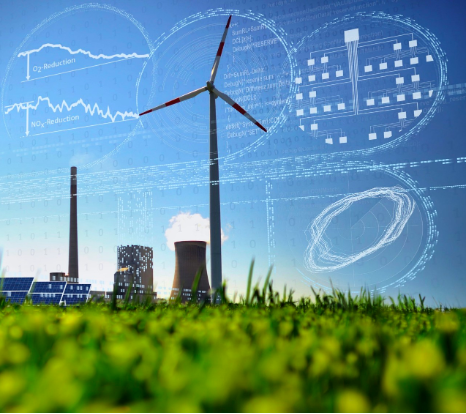
\includegraphics[width=0.6\textwidth, clip, trim={0cm 0cm 0cm 0cm}]{FrontMatter/Cover/Cover}}
                        }
                        %        	\vspace*{1.0cm}
                \end{figure}



                %% Additional whitespace for ease of eye
                \vspace*{2\bigskipamount}


                %% Text color is changed for readability
                \color{white}

                %% Print the name of the author.
                {\makeatletter
                        \largetitlefont\Large\bfseries
                        \largetitlestyle\fontsize{24}{13cm}\selectfont Utrecht University
                        \makeatother}


                %% Additional whitespace for ease of eye
                \vspace*{2\bigskipamount}
        \end{center}


% \end{titlepage}

%% Print an overview of the layout
%\layout

\end{document}


